\documentclass{whutmod}
\usepackage{metalogo}
\usepackage{float}
\usepackage{subfigure} 
\usepackage{url}
\usepackage{booktabs}
\bibliographystyle{unsrt}
\team{23}
\membera{刘子川}
\joba{编程}
\memberb{程宇}
\jobb{建模}
\memberc{陈荣兴}
\jobc{建模}
\hypersetup{
	colorlinks=true,
	linkcolor=black
}

\title{基于因子分析与灰色关联分析对武汉市人才吸引力的量化评价}
\tihao{4} 

\begin{document}

	%\maketitle
	
	\begin{abstract}

%植物的种类繁多,为研究植物分类方法,本文基于植物树叶的二值化图片数据,通过\textbf{解析几何计算}和\textbf{时间序列展开}的方法转换成轮廓特征向量和边缘特征向量;再通过\textbf{粒子群算法}优化的\textbf{深度神经网络}解决树叶识别分类问题,并分析核心指标对模型性能的影响,最终结合树叶纹理信息对模型进行改进和分析比较。
~\\

针对问题一,将原问题转化成多背包优化问题,建立了\textbf{最少船舰数量装载模型},求解得到装备人口装载方案。根据题目要求,首先对兵力、装备与船载的面积进行量化,得到相关的面积向量。然后建立船舰数量的决策向量,并结合题中相关条件和要求,对函数模型进行约束与优化。自创\textbf{沙石算法},进行装备均分和部队装载,求解得到各旅级单位装备人口的面积装载方案和各类舰船的使用数量。各类船舰的有效面积利用率基本达到$\textbf{90\%}$以上。
~\\


%针对问题二,基于问题一中提取的特征信息,建立了\textbf{PSO-DNN网络}对树叶进行识别与分类。利用\textbf{Keras工具库}搭建\textbf{深度神经网络},利用\textbf{粒子群算法}优化DNN网络的连接权值和阈值,对研究对象进行识别分类。训练后的神经网络模型预测准确率为$\textbf{91.037\%}$,并分析各指标的权重占比,判断出特征量中\textbf{时间序列熵、密实度和最大压痕深度}对模型性能影响最大,是模型的核心指标。将其剔除后,模型分类精确度损失率分别为\textbf{6.937\%、5.498\%、3.559\%}。
~\\

%针对问题三,基于问题二中的\textbf{PSO-DNN网络}模型,将树叶纹理信息嵌入特征向量。增加网络输入层个数,并对模型进行参数调整,最终得到叶片的预测准确率达到$\textbf{96.634\%}$。
~\\

本文中的模型优势主要有两点:一是自主设计沙石算法,使得船舰的面积利用率高,对船只数量的需求量少;二是使用遗传算法,运算时间相较于全遍历算法更短,具有很强的全局搜索能力和鲁棒性,
	
  
\keywords{沙石算法\quad 遗传算法\quad  粒子群算法\quad Keras工具库\quad }
		
	\end{abstract}
	
	%目录
	\tableofcontents
	\newpage	%换页符
	
	\section{问题重述}	
	\subsection{问题背景}
    诺曼底登陆:代号“霸王行动”,是第二次世界大战中盟军在欧洲西线战场发起的一场大规模攻势,接近三百万士兵渡过英吉利海峡前往法国诺曼底。诺曼底战役是人类战争史上规模最大的一次海上登陆战役行动,使第二次世界大战的战略态势发生了根本性的变化。
    
    海运装载是海上登陆战役中的一种作战行动,将需要登陆的部队人员、装备、补给品装载到海上运输工具,该行动会直接影响着登陆作战效果。以诺曼底战役的第一批海上登陆输送兵力为参考,不同成建制单位的部队人员、装备和补给品都有不同的数量级需求,研究合理利用海军运输船和民用船只进行兵力装载以及对装载方案的优化都具有重要意义。
    
    
    

	\subsection{问题概述}
    围绕相关附件和条件要求,研究海运装载行动输送兵力任务的合理安排,依次提出以下问题:
		 
	
	\textbf{问题一:}根据输送任务和海上运输工具情况,结合相关条件和要求,分析运输船舰和兵力的关系,概算各类型旅一个旅级单位的运输工具的需求量,并给出具体装载方案。
	
	\textbf{问题二:}根据输送任务,结合附件中的港口及码头泊位,制定时间最短、船只数量最少的兵力装载方案。
	
	\textbf{问题三:}假设装载行动开始24小时后,A港口的两个A1和一个A2泊位,D港口的一个D2和两个D3泊位被毁,给出具体调整方案以及完成装载任务的对策建议。
	
	
	\section{模型假设}
	\begin{itemize}                                             
		\item [(1)] 为了简化计算,假设题目中给出的模糊数据都是精确数据。
		\item [(2)] 为了优化运算结果,假设所有全副武装的士兵都保持坐姿休息。
		\item [(3)] 假设在战争中,装载消耗更少时间的优先度高于使用更少的民用船。
		\item [(4)] 假设在装载过程中,同一泊口的船舰装载交替时间可以忽略不记。
		\item [(5)] 假设港口被摧毁时,由于提前得到信息,港口上的船只与兵力没有损失,只是正在进行的装载工作停止,且进度完全损失。
	\end{itemize}
	
	
	\section{符号说明}
	\begin{table}[H]
	\label{biao} \centering

	\begin{tabular}{cc}
		\toprule[1.5pt]
		\multicolumn{1}{m{5cm}}{\centering 符号} & \multicolumn{1}{m{5cm}}{\centering 说明} \\
		\midrule[1pt]		
		$X_{i}$  &  第i型装备 \\ 
		$s_{xi}$  &  装备$X_{i}$的占用面积 \\ 
		$l_{i}$  & 装备$X_{i}$的长\\
		$w_{i}$  &  装备$X_{i}$的宽 \\ 
		$\varepsilon _{i}$ & 装备$X_{i}$的面积修正系数\\
		$p_{i}$	 &  全副武装人员数  \\ 
		$eta_{1}$ &  海军船舰的有效面积率 \\ 
		$eta_{2}$	 &  民用船只的有效面积率 \\ 
		$y_{k}$  &   登陆舰数量\\ 
		$z_{n}$  &  民用船数量\\	
		$D$ & 决策向量\\
		$S_{D}$ &  舰载面积系数向量\\ 
		$S_{z}$ & 民用船有效面积向量\\
		$S_{y}$ & 登陆舰有效面积向量\\
		$S_{p}$ & 每营人口面积向量\\
		$A^{k}$  & 面积规划向量\\
		$T_{n}$ & 颖编制总部对数列\\
		$P_{n}$ & 船舰面积数列\\
		$\eta $ &  平均有效面积利用率\\

		\bottomrule[1.5pt]
	\end{tabular}
\end{table}

	\section{问题一模型的建立与求解}

    \subsection{问题描述与分析}

    问题一要求根据输送任务和船舰情况,结合相关条件和要求,分析运输船舰和兵力的关系,概算各类型旅一个旅级单位对船舰的需求量,给出装载方案。其本质是一个多背包优化问题,要求使用尽可能少的背包,装载各种旅的一个旅编制兵力。本组首先对兵力、装备与装载的面积进行量化,根据题目要求,以派出船舰种类和数量作为决策向量,以所用的总船只数量为目标函数,设计沙石算法,使得每艘船面积利用率达到最高,从而调用船支数达到最小值。
    

	    \subsection{模型的建立}
	    \subsubsection{兵力、装备与船载的面积量化}


	    计算附件2中的每种装备与所占面积,得到装备占用面积向量:
	    \begin{gather*}
	    s_{xi}=l_{i}\times w_{i} \times \varepsilon _{i}\\
	        S_{x}=[s_{x1},s_{x2},\cdots,s_{x14}]
	    \end{gather*}
	    其中$s_{xi}$是装备$X_{i}(i=1,2\cdots,14)$的占用面积,$l_{i}$、$w_{i}$与$\varepsilon _{i}$分别是装备$X_{i}$的长、宽与面积修正系数。
	    
	     计算附件2中每种旅一个营的占用面积,得到每营人口所占面积向量:


	     \begin{gather*}
	     s_{pi}=p_{i}\times s\\
	     S_{p}=[s_{p1},s_{p2},\cdots,s_{p12}]
	     \end{gather*}
	     其中$p_{i}$是第$i(i=1,2,\cdots,12)$的全副武装人员数,取$s=0.5m^2$为每个全副武装人员占用的面积。
	     
	     计算附件3中登陆舰可用装载面积,得到登陆舰有效面积向量:
	      \begin{gather*}
	      s_{yi}=s_{i}\times \eta_{1}\\
	      S_{y}=[s_{y1},s_{y2},\cdots,s_{y14}]
	      \end{gather*}
	    其中$s_{yi}$是登陆舰$Y_{i}(i=1,2\cdots,14)$的可用装载面积,$s_{i}$是登陆舰$Y_{i}$的总装载面积,取$\eta_{1}=75\%$为登陆舰的有效面积率。
	    
	    计算附件3中民用船可用装载面积,得到民用船有效面积向量:
	      \begin{gather*}
	      s_{zj}=s_{j}\times \eta_{2}\\
	      S_{z}=[s_{z1},s_{z2},\cdots,s_{z5}]
	      \end{gather*}
	       其中$s_{zi}$民用船$Z_{j}(i=1,2\cdots,5)$的可用装载面积,$s_{j}$是民用船$Z_{j}$的总装载面积,取$\eta_{2}=70\%$为民用船只的有效面积率。
	    \subsubsection{优化函数与约束条件}
	    令$y_{k} $ $(k=1,2,\cdots ,14)$为派出的登陆舰数量,$z_{n}$$(n=1,2,\cdots ,5)$为派出民用船的数量,建立\textbf{决策向量}:
	     \begin{gather*}
	     D=[y_{1},y_{2},\cdots,y_{14},z_{1},z_{2},\cdots,z_{5}]
	    \end{gather*}
	    
	    
	    根据题意尽可能使用少的船舰数,即\textbf{目标函数}为使用船舰总数:
	     \begin{gather}
	    min Z=\sum _{1}^{19}D[k]
	  \end{gather}
	    
	    
	   其中舰载面积系数向量为:
	    \begin{gather*}
	    S_{D}=[S_{y}, S_{z}]
    	\end{gather*}
    	
    	根据题目要求总舰载有效面积不小于总兵力装备占用面积:
    	 \begin{gather*}
    	 D\cdot S_{D}\geq \sum  S_{x} + \sum  S_{p}
    	 \end{gather*}
    	 
    	 且由登陆舰Y1的有效舰载面积大于装备X9(直升机)的部队占用的面积,其中$\sum  s_{p6}$是唯一装备的部队—$\uppercase\expandafter{\romannumeral6}$旅的人口总和:
    	  \begin{gather*}
    	 y_{1}\cdot s_{y1}\geq \sum s_{x9}+ \sum  s_{p6}
    	 \end{gather*}
    	 
    	 

    	 综上,建立得到使用最少船舰装载每种旅各一个旅级编制的\textbf{模型}为:
    	  \begin{gather}
\begin{matrix}
minZ=\sum _{1}^{19}D[k]
\\
\\
s.t.\left\{\begin{matrix}	 D\cdot S_{D}\geq \sum  S_{x} + \sum  S_{p}
\\ y_{1}\cdot s_{y1}\geq \sum s_{x9}+ \sum  s_{p6}
\\S_{D}=[S_{y}, S_{z}]
\\ s_{xi}=l_{i}\times w_{i} \times \varepsilon _{i}
\\S_{x}=[s_{x1},s_{x2},\cdots,s_{x14}]
\\s_{pi}=p_{i}\times s
\\S_{p}=[s_{p1},s_{p2},\cdots,s_{p12}]
\\     s_{yi}=s_{i}\times \eta_{1}
\\   S_{y}=[s_{y1},s_{y2},\cdots,s_{y14}]
\\      s_{zj}=s_{j}\times \eta_{2}
\\ S_{z}=[s_{z1},s_{z2},\cdots,s_{z5}]
\end{matrix}\right.
\end{matrix}
     	 \end{gather}

    		    	
	\subsection{模型的求解}   
    	  \subsubsection{沙石算法}

		为使得调用的船舰数量最少,即需使得每艘船的未利用面积值达到最小:
	    \begin{gather}
		min \Delta S= \sum  S_{x} + \sum  S_{p}-D\cdot S_{D} 
		\end{gather}
	其中$\Delta S$为损失面积,本组设计沙石算法优化部队装载方案,使其得面积损失达到最小,具体如下:
	 \paragraph{算法思想}
	 根据经验,使用沙砾和石子填满某个刚性容器,较好的方法是先装入石子,后灌入沙砾,可以让剩余空间达到最小。基于此,本组设计\textbf{沙石算法},将带待装载部队(其占用面积不尽相同)视作沙砾与石子,将船舰视作刚性容器,即可求出面积利用率最高的部队装载方案。沙石算法示意图如图 ~\ref{shashi}~所示:
	 
	 
	 \begin{figure}[H]
	 	\centering
	 	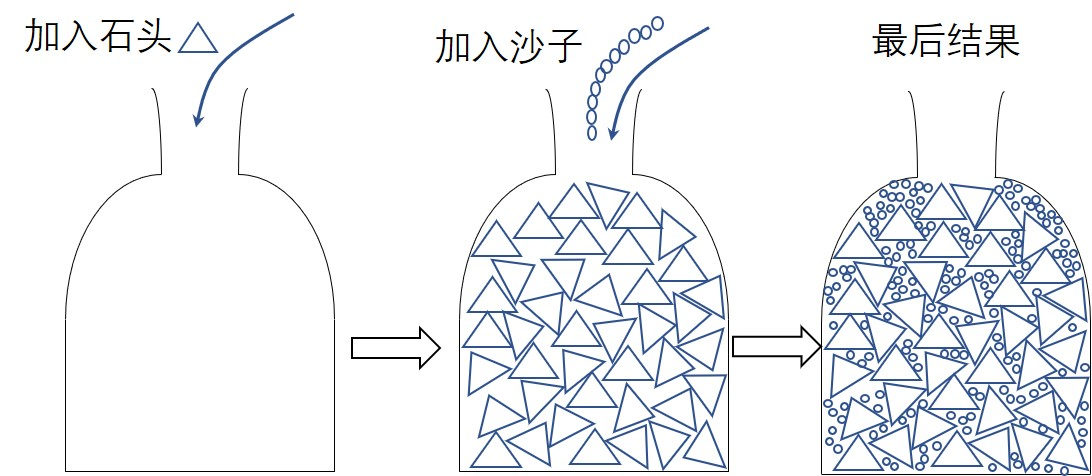
\includegraphics[width=.8\textwidth]{figures/shashi.jpg}
	 	\caption{沙石算法示意图}\label{shashi}
	 \end{figure}
	 
	 \paragraph{算法描述}
	 	\begin{itemize}
	 	\item [(1)] \textbf{装备均分}:将每个旅分解为连编制,即得到面积规划向量:
	 \begin{gather*}
	 	A^k=[a^k_{1},a^k_{2},\cdots,a^k_{n}]
	\end{gather*}
	 	其中$a^k_{i}$的初始值是第$k$旅中的全副武装人员所占面积,$k=1,2,\cdots,K$($K$为旅队编制总数),$n=n_{k}$($n_{k}$为$k$旅连编制总数)。根据题目中装备均匀分配的要求,重复检索向量$A^k$中的每一个元素,选择最小值$min \left \{ a_{i} \right \}$ (装备量最少的营)使得该连添加装备$X_{j}$,即令:
	 	\begin{gather*}
	   min \left \{ a_{i} \right \}=min \left \{ a_{i} \right \}+s_{xj}
	 	\end{gather*}
	 	重复检索直到该旅装备数$X=0$时,结束装备均分,得到装备均分后的部队$ \left \{A^k\right \}(k=1,2,\cdots,n_{k})$($n_{k}$为k旅连编制总数)。
	
		\item [(2)] \textbf{部队装载}:将装备均分后的部队$ \left \{A^k\right \}$中的元素混合后由大到小进行排序得到排序后的营编制总部对数列$ \left \{T_{n}\right \}$:
			\begin{gather*}
	T_{n}\geqslant 	T_{n+1}\\
	n\leq \sum_{1}^{K}n_{k}
		\end{gather*}
		将所有派出船舰装载面积进行排序得到船舰面积数列$ \left \{P_{n}\right \}$:
		依次检索总部对数列$ \left \{T_{n}\right \}$,并依次检索数列$ \left \{P_{n}\right \}$对应的船舰,将其装入剩余面积足够的船舰,即若$P_{n}\geqslant T_{n}$ 令:
		\begin{gather*}
		P_{n}=	P_{n}-	T_{n}
		\end{gather*}
		重复检索直到部队装载完成,即当部队检索次数$i=\sum_{1}^{K}n_{k}$时,算法结束。
		\item [(3)] \textbf{结果输出}:输出总共使用的船舰数量,即决策向量:
		\begin{gather*}
		D=[y_{1},y_{2},\cdots,y_{14},z_{1},z_{2},\cdots,z_{5}]
		\end{gather*}
	\end{itemize}
	%沙石算法的流程图如图~\ref{shashiluc}~
	 
\begin{figure}[H]
	\centering
	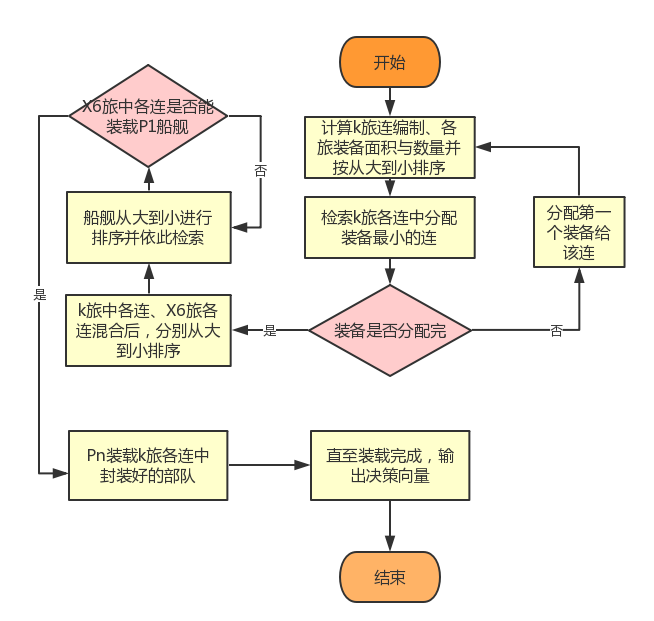
\includegraphics[width=.9\textwidth]{figures/shashisuanfa.png}
	\caption{沙石算法流程图}\label{shashiluc}
\end{figure}


\subsection{结果分析}
通过量化各型旅成建制单位的人数、装备面积和船舰的有效装载面积,结合相关条件和要求,再运用沙石算法进行计算,求解出各旅级单位装备人口面积装载方案如表~\ref{zhuangzai}~,其各连对应的某种装备具体到每艘轮船数据见附件:

\begin{table}[H]
\centering		\caption{各型旅级单位装备人口面积装载方案}\label{zhuangzai}
\begin{tabular}{cccccc}
	\toprule[2pt]
	\multicolumn{1}{m{2cm}}{\centering 船舰类别}
	& \multicolumn{1}{m{2cm}}{\centering 第Ⅰ型旅}
	&\multicolumn{1}{m{2cm}}{\centering 第Ⅱ型旅}
	& \multicolumn{1}{m{3cm}}{\centering $ \cdots \cdots  $}
	& \multicolumn{1}{m{2cm}}{\centering 第Ⅺ型旅}
	& \multicolumn{1}{m{2cm}}{\centering 第Ⅻ型支队(旅)}
	\\
	\midrule[1pt]
	Y1综合登陆舰 &  $267.6285185$  &$0$ & $\cdots \cdots$&$5658.770914
	$ &$42.85714286$ \\ 
	Y2大型登陆舰	 &  $1586.951111$&$0$& $\cdots \cdots$ &$0$ &$0$\\ 
	Y3大型登陆舰	 &  $3178.042222 $ &$0$& $\cdots \cdots$ &$5864.014286
	$ &$0$\\ 
	Y4大型登陆舰	 &  $2114.508148 $ &$0$& $\cdots \cdots$ &$0
	$ &$0$\\ 
	Y5大型登陆舰	 &$5621.115$ &$0$& $\cdots \cdots$ &$0
	$ &$385.714$\\
	Y6中型登陆舰	 &$492.417$ &$3557.613$& $\cdots \cdots$ &$0
	$ &$0$\\
	Y7中型登陆舰	 &$0$ &$438.3834$& $\cdots \cdots$ &$0
	$ &$0$\\
	Y8中型登陆舰	 &$793.7356$ &$0$& $\cdots \cdots$ &$0
	$ &$0$\\
	Y9中型登陆舰	 &$0$ &$1468.704$& $\cdots \cdots$ &$0
	$ &$342.8571$\\
	Y10中型登陆舰	 &$0$ &$0$ & $\cdots \cdots$ &$0
	$ &$0$ \\
	Y11登陆舰	 &$0$ &$0$& $\cdots \cdots$ &$0$ &$0$ \\
	Y12登陆艇	 &  $0$ &$0$ & $\cdots \cdots$ &$0$ &$728.5714286$\\ 
	Y13登陆艇	 &  $0$ &$0$ & $\cdots \cdots$ &$0$ &$0$\\ 
	Y14登陆艇		 &  $0$ &$0$ & $\cdots \cdots$ &$0$ &$0$\\ 
	2万吨级滚装船  &  $0 $ &$6549.897037$& $\cdots \cdots$ &$0$ &$0$ \\ 
	\bottomrule[2pt]	
\end{tabular}
\end{table}

	其种各类舰船的使用数量$num$与平均有效面积利用率$\eta=\frac{\sum P_{n}\cdot S_{k}}{\sum D*S_{n}*0.75}$,计算结果如表~\ref{zhuansasgzai}~所示。可以见的,其沙石算法设计的装备兵力装载方案\textbf{有效面积利用率相当高},能最大程度的\textbf{利用最少的船只数目}填充更多武装兵力。在实际作战中,将建制单位细化至连并计算修正面积,再进行"沙石"思想的封装进船舰后,能大幅度减小船舰使用数目,以达到装载行动迅速高效的目的。
	\begin{table}[H]
		\centering		\caption{各类舰船的使用数量与平均有效面积利用率}\label{zhuansasgzai}
		\begin{tabular}{ccc}
			\toprule[2pt]
			\multicolumn{1}{m{3cm}}{\centering 船舰类别}
			& \multicolumn{1}{m{3cm}}{\centering 使用数量}
			&\multicolumn{1}{m{3cm}}{\centering 平均有效面积利用率}
			\\
			\midrule[1pt]
			Y1综合登陆舰 &  $5$  &$99.25$\% \\ 
			Y2大型登陆舰	 &  $3$&$94.04$\%\\ 
			Y3大型登陆舰	 &  $9 $ &$99.81$\%\\ 
			Y4大型登陆舰	 &  $4$ &$93.98$\%\\ 
			$\cdots \cdots$	 & 	$\cdots \cdots$&	$\cdots \cdots$\\ 
			Y12登陆艇	 &  $138$ &$70.38$\%\\ 
			2万吨级滚装船  &  $1 $ &$93.74$\% \\ 
			\bottomrule[2pt]	
		\end{tabular}
	\end{table}

	
	
		
	\section{问题二模型的建立与求解}
	\subsection{问题的描述与分析}

	问题二要求针对具体运输任务,结合港口泊位,制定时间最短、船只数量最少的兵力装载方案。本组通过\textbf{遗传算法},将问题一中的决策向量作为染色体,装载时间和船支数量作为适应度函数,建立装载方案优化模型。修改问题一中的\textbf{沙石算法},作为验证算法判断每个个体是否可以存活,并随机生成$w$个能通过验证算法的初始个体。将某一代个体经过交叉、变异后的基因带入\textbf{时间轴仿真模型},计算出装载所用时间作为适应度函数,将生成个体按照适应度函数大小进行第一次排序,再将装载所用时间大小相同的函数进行第二次排序,取出排序中前$w$个个体进行下一次进化,进化$g$代个体后可求得\textbf{装载时间最短、使用海上运输工具最少}的兵力装载方案。	                                                                                                   
	\subsection{模型的建立}
	    \subsubsection{优化函数与约束条件}
	基于问题一模型\textbf{决策向量}为:
	\begin{gather*}
	D=[y_{1},y_{2},\cdots,y_{14},z_{1},z_{2},\cdots,z_{5}]
	\end{gather*}
	\textbf{目标函数}为:
	\begin{gather}
	min Z=\sum _{1}^{19}D[k]
	\end{gather}
	增加\textbf{目标函数}:
		\begin{gather}
	min \left \{ \underset{k}{max}\sum t_{i} \right \}
	\end{gather}
	其中$\sum t_{i}(i=1,2\cdots,71)$,表示在共计$71$个泊口中第$i$个泊口的装载时间总和。	
	

	且由于集装箱船(Z3)无法装载装备X1,X2,X3和X4,增加	\textbf{约束条件}:
	\begin{gather}
	D \cdot S_{D} - z_{3} \cdot s_{z3} \geq  \sum s_{x1}+ \sum s_{x2}+\sum s_{x3}+ \sum s_{x4}
	\end{gather}
	
	
		综上,建立得到问题二\textbf{时间与船数优化模型}:

	\begin{gather}
min Z=\sum _{1}^{19}D[k]\\
min \left \{ \underset{k}{max}\sum t_{i} \right \}\\
s.t.\left\{\begin{matrix}	 D\cdot S_{D}\geq \sum  S_{x} + \sum  S_{p}
\\ y_{1}\cdot s_{y1}\geq \sum s_{x9}+ \sum  s_{p6}
\\S_{D}=[S_{y}, S_{z}]
\\ s_{xi}=l_{i}\times w_{i} \times \varepsilon _{i}
\\S_{x}=[s_{x1},s_{x2},\cdots,s_{x14}]
\\s_{pi}=p_{i}\times s
\\S_{p}=[s_{p1},s_{p2},\cdots,s_{p12}]
\\     s_{yi}=s_{i}\times \eta_{1}
\\   S_{y}=[s_{y1},s_{y2},\cdots,s_{y14}]
\\      s_{zj}=s_{j}\times \eta_{2}
\\ S_{z}=[s_{z1},s_{z2},\cdots,s_{z5}]
\\	D \cdot S_{D} - z_{3} \cdot s_{z3} \geq  \sum s_{x1}+ \sum s_{x2}+\sum s_{x3}+ \sum s_{x4}
\end{matrix}\right. 
\end{gather}
	     ~\\
	其中$ \underset{k}{max}\sum t_{i} $可利用\textbf{泊口仿真模型}计算,并通过\textbf{遗传算法}算得全局最优解。
	\subsubsection{泊口仿真模型}
	建立泊口仿真模型以计算每种方案的装载时间,首先输入决策向量:

		\begin{gather*}
	 D=[y_{1},y_{2},\cdots,y_{14},z_{1},z_{2},\cdots,z_{5}]
		\end{gather*}
	定义时间函数为$t_{0}$,初始化时间函数令$t_{0}=0$,并令$t_{0}$以$1$为步长逐渐增加。
	定义港口决策向量为:
		\begin{gather*}
		T=[t_{1},t_{2},\cdots,t_{71}]
		\end{gather*}
	$t_{k}(k=1,2,3,\cdots,71)$代表$71$个港口当前任务的结束时间。当$t_{k}=t_{0}$ 时,表示港口$k$处于空闲状态,此时立即更新任务结束时间$t_{k}$,即使得:
		\begin{gather*}
		t_{k}=t_{k}+t_{d}\\
		D[d]=D[d]-1
		\end{gather*}
	其中$t_{d}$是决策向量$D$中第$d$各元素对应船舰的装载时间,$D[d]$为决策向量$D$中的第$d$个元素。当
		\begin{gather*}
	\left\{\begin{matrix} \sum_{1}^{19}D[d]=0
	\\t_{0}\geqslant max t_{k} 	
	\end{matrix}\right.
		\end{gather*}

		即所有船支装载完成时,结束运算,输出当前的时间函数$t_{0}$,即:
			\begin{gather*}
		min \left \{ \underset{k}{max}\sum t_{i} \right \}=t_{0}
			\end{gather*}
    \begin{figure}[H]
	\centering
	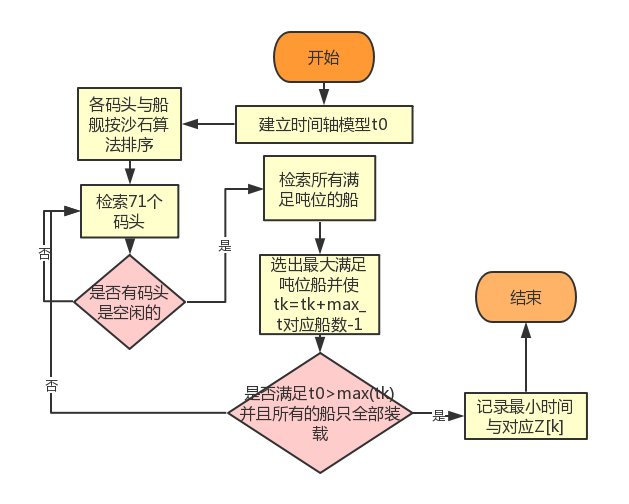
\includegraphics[width=.9\textwidth]{figures/yyy.png}
	\caption{泊口仿真流程图}\label{dieyyrwen}
\end{figure}
	\subsubsection{遗传算法}
	 \paragraph{编码}
	 如图所示,每个个体由下面三个方块构成,其中最后一个进行遗传操作:
	 	\begin{figure}[H]
	 	\centering
	 	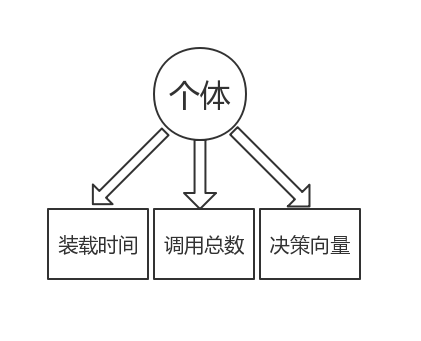
\includegraphics[width=.5\textwidth]{figures/yichuan.jpg}
	 	\caption{指标重要度占权图}\label{yichuan}
	 	 \end{figure}
	 根据题目要求,优先使用军用登陆舰,即决策向量$D=[y_{1},\cdots,y_{14},z_{1},\cdots,z_{5}]$中$y_{k}(k=1,2,\cdots,14)$为恒定值且等于其上限。故能简化决策向量为:
	\begin{gather*}
	D=[z_{1},z_{2}\cdots,z_{5}]
	\end{gather*}
	 \paragraph{交叉}
	 为保证变异率并保留优秀基因片段和本题采用的两种交叉方式:
	\begin{itemize}
	\item [(1)]单点交叉:对于两个父代个体$D=[z_{1},z_{2}\cdots,z_{5}]$和	$D'=[z_{1}',z_{2}'\cdots,z_{5}']$,随机选择第$k$个基因处为交叉点,将该基因后所有基因进行交换,得到子代基因
	\item [(2)]中间值交叉:对于两个父代个体$D=[z_{1},z_{2}\cdots,z_{5}]$和	$D'=[z_{1}',z_{2}'\cdots,z_{5}']$,随机选取$z_{k}''\in [z_{k},z_{k}']$得到子代基因。
    \end{itemize}
    再选取交叉个体时采用混合分组的方法,将父代均匀混合后选取所有编号为奇数的个体,与其相邻对应编号为偶数的个体,通过两种交叉方式产生处两种类型的子代。
     \paragraph{变异}
     为保证种群多样性,以$0.1$的变异率,对选择的个体执行变异操作。随机选择变异个体中的基因$z_{k}$,使其值以各$50\%$的概率加一或减一。
     \paragraph{筛重}
     由于该模型基因维度较低,有大概率出现基因重复的个体,其对种群多样性有不利影响,并易使算法早熟。故在每次交叉变异生成新个体时删除重复基因,以提高算法的全局搜素能力。
     \paragraph{选择}
     由于本题约束条件较多,且有两个包含两个适应度函数,故采用两种选择方式:
     \begin{itemize}
     \item [(1)] \textbf{约束淘汰:}对于生成的个体基因$D=[z_{1},z_{2}\cdots,z_{5}]$带入第一问的沙石算法中,计算部队是否可以完全装入船支中。若不能则删除个体,若能则保留个体。
     \item [(2)]\textbf{精英选择:}由于模型假设战场上使用较少的时间优先级高于使用更少船支,将每一代中的生成个体与上一代混合,的个体按照其\textbf{装载时间}由大到小进行\textbf{第一次排序},再将装载时间相同的个体进行依照\textbf{调用总数}进行\textbf{第二次排序}。保留前列的$w$个个体,$w$为设定的种群容纳量。
     \end{itemize}
     重复上述进化过程,当进化代数足够多时,求解得到全局最优解。

     \subsection{模型求解与算法实现}


   	 (1) 将染色体中的单个基因取出,带入问题一沙石算法中。计算只使用的某种民用船时,需要的该民用船的数量,作为单个基因的取值范围。在使用卡特蒙洛法随机生成初始个体,当生成$50$个能通过沙石算法检验的初始个体时,停止生成。
   	 (2)将输入体进行、交叉、变异、筛重和约束淘汰后,得到子代生成个体。将子代个体与附带个体混合,带入泊口仿真模型求出每个个体的装载时间作为适应度函数。根据装载时间对每个个体进行第一次排序,并将装载时间相同的个体进行第二次排序,取序列中的前$50$个个体作为下一代输入个体。

   (3)重复上述步骤(2),当进化次数达到$100$次时结束进化,选取当前最优个体作为输出的个体,将输出个体基因与军用登陆舰总调遣数量合并即可得到完整的船支调遣方案。


    	 
    	 其求解该模型的具体流程图如~\ref{dierwen}~所示:
    \begin{figure}[H]
    	\centering
    	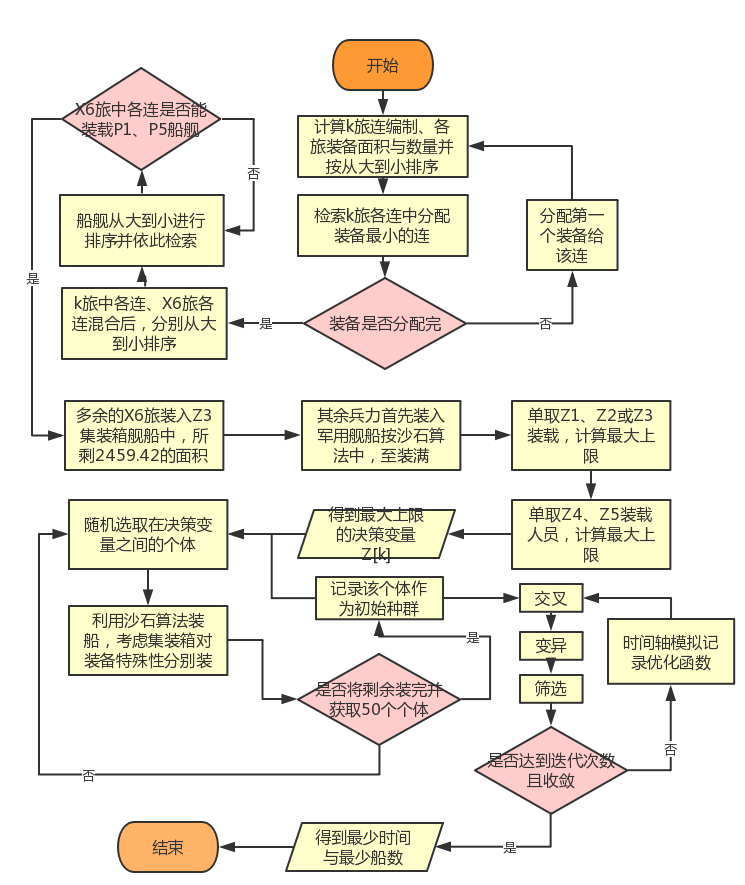
\includegraphics[width=\textwidth]{figures/dierwen.png}
    	\caption{沙石遗传算法与时间轴仿真流程图}\label{dierwen}
    \end{figure}
     
     	\subsection{结果分析}
     \section{问题三模型的建立与求解}
   	\subsection{问题的描述与分析}
   	问题三要求,当装载行动开始24小时后,A港和D港有部分泊位被毁,给出调整方案和装载建议。
   	本组基于问题二中模型求解的结果,作出合理假设,假设泊位被毁不损失船只和兵力,由于问题二中的装载时间最优解小于$24$小时,根据建议将码头被摧毁时间改为第$18$小时。本组延用问题二中的遗传算法,当时间轴进行到$18$小时,剔除已经完成装载任务的船舰和A港、D港中部分被毁的码头泊位,修改问题二中的港口仿真模型。通过遗传算法求解出对剩余船舰、码头泊位的装载方案,给出装载建议。
  \subsection{模型的建立}
    \subsubsection{模型调整}
    \textbf{优化函数与约束条件}延用问题二模型:
     	\begin{gather}
min Z=\sum _{1}^{19}D[k]\\
min \left \{ \underset{k}{max}\sum t_{i} \right \}\\
s.t.\left\{\begin{matrix}	 D\cdot S_{D}\geq \sum  S_{x} + \sum  S_{p}
\\ y_{1}\cdot s_{y1}\geq \sum s_{x9}+ \sum  s_{p6}
\\S_{D}=[S_{y}, S_{z}]
\\ s_{xi}=l_{i}\times w_{i} \times \varepsilon _{i}
\\S_{x}=[s_{x1},s_{x2},\cdots,s_{x14}]
\\s_{pi}=p_{i}\times s
\\S_{p}=[s_{p1},s_{p2},\cdots,s_{p12}]
\\     s_{yi}=s_{i}\times \eta_{1}
\\   S_{y}=[s_{y1},s_{y2},\cdots,s_{y14}]
\\      s_{zj}=s_{j}\times \eta_{2}
\\ S_{z}=[s_{z1},s_{z2},\cdots,s_{z5}]
\\	D \cdot S_{D} - z_{3} \cdot s_{z3} \geq  \sum s_{x1}+ \sum s_{x2}+\sum s_{x3}+ \sum s_{x4}
\end{matrix}\right. 
\end{gather}
     ~\\
     调整 \textbf{泊口仿真模型},延用港口决策向量:
     \begin{gather*}
     T=[t_{1},t_{2},\cdots,t_{71}]
     \end{gather*}
     当时间轴函数$t_{0}=18$时,停止被毁泊口正在进行的任务,使得:
     \begin{gather}
     \left\{\begin{matrix}
     t_{k}=-1(k=1,2,11,37,46,47)\\ 
     D[d]=D[d]+1
     \end{matrix}\right.
     \end{gather}
     即立刻终止港口正在进行的工作,且在$18$小时后检索港口决策向量时,剔除$t_{k}(k=1,2,11,37,46,47)$(其对应被摧毁的港口无法执行装载任务)。并将修改后泊口仿真模型算得的装载时间,带入遗传算法的适应度函数值,重新运行遗传算法。即可求得装载中途港口被摧毁后的最优船舰调整方案。
       \subsection{模型的求解}
     \paragraph{算法的实现}

	沿用第二问算法,仅修改泊口仿真模型:如果达到摧毁时间,将第$i$个摧毁港口的任务结束时间$t_{ki}$修改为$-1$,并不再更新此港口。若此时港口$i$不是空闲港口,将对应船舰$d_{i}$的数目增加一个。其算法流程图如下:
    \begin{figure}[H]
	\centering
	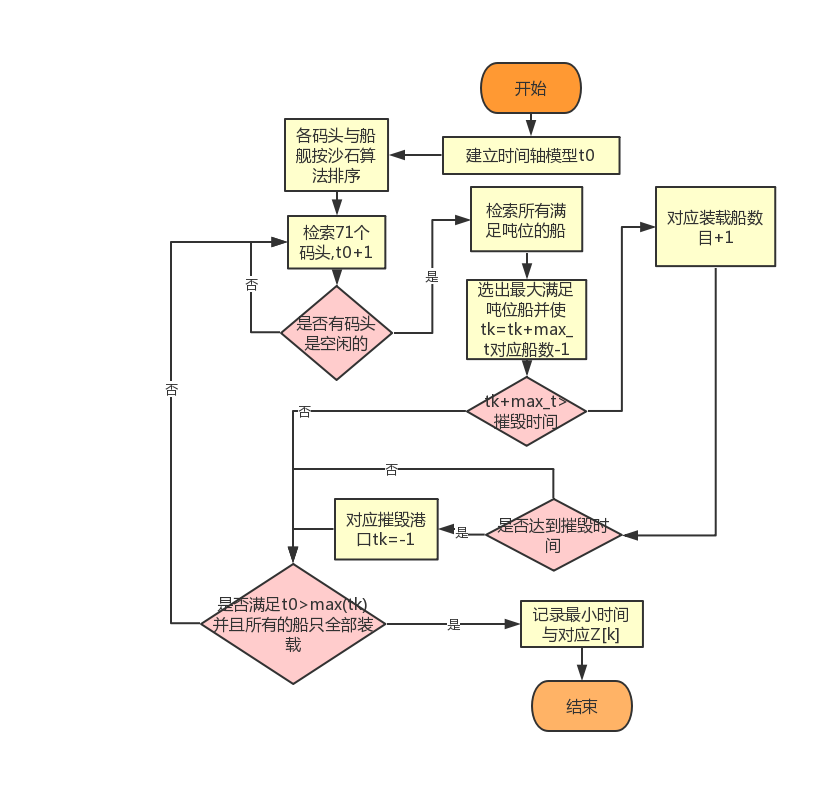
\includegraphics[width=\textwidth]{figures/yyyy.png}
	\caption{泊口仿真改进流程图}\label{dieyyrywen}
\end{figure}

	

	
	\subsection{结果分析}
     



	\section{模型的评价}
	\subsection{模型的优点}
		\begin{itemize}                                             

		\item [(1)] 将多目标优化转换成背包优化问题,自主设计沙石算法,使得船舰的面积利用率高,对船只数量的需求量少。
		\item [(2)] 使用遗传算法,具有很强的全局搜索能力和鲁棒性,运算时间远小于全遍历算法。
	\end{itemize}
	\subsection{模型的缺点}

	遗传算法初始解由卡特蒙洛法随机生成,每次搜索结果不完全相同,可能引起结果的偏差,需要多搜索几次选择才能得到最优结果。
	\subsection{模型改进}
	可使用改进的生命遗传算法,加强算法的局部搜索能力,解决算法早熟的问题。

 
	\newpage	%换页符
	%%参考文献
	%\begin{thebibliography}{9}%宽度9
	% \setlength{\itemsep}{-2mm}
	\nocite{*}		%排版未引用的参考文献
%\bibliography{wenxian.bib}
%	%参考文献添加到wenxian.bib里,再引用
%	
\begin{thebibliography}{9}%宽度9
	\bibitem{bib:one}Febri Liantoni,Rifki Indra Perwira,Syahri Muharom,Riza Agung Firmansyah,Akhmad Fahruzi. Leaf classification with improved image feature based on the seven moment invariant[J]. Journal of Physics: Conference Series,2019,1175(1).

\end{thebibliography}

	\newpage
	%附录
	\appendix %%附录

\section{代码}
\subsection{问题一沙石算法--python源代码}
\begin{lstlisting}[language=python]
import math
import numpy as np
import pandas as pd


def append(list,x):
'''numpy数组中插入一个元素在末尾'''
return np.append(list,x)


def Merge(dict1, dict2):
'''字典合并'''
res = {**dict1, **dict2}
return res


def shell_sort(lists):
'''
按从大到小排序,时间复杂度O(n)
:param lists:传进来的数组,比如船只或者包裹
:return: 返回从大到小的包裹
'''
# 希尔排序
lists = sorted(lists,reverse=True)
return lists


def kv_sort(kv):
'''
键值对由大到小排序
eg:
d = {'d1':2, 'd2':4, 'd4':1,'d3':3,}
res = sorted(d.items(),key=lambda d:d[1],reverse=True)
[('d2', 4), ('d3', 3), ('d1', 2), ('d4', 1)]
:param kv:键值对
:return:元组
'''
res = sorted(kv.items(), key=lambda d: d[1], reverse=True)
return res


def min_index(lists):
'''
返回最穷连的下标
:param lists: 各连的装备面积数目
:return: 最穷的那个连的下标
'''
index_min = 0
for i in range(1, len(lists)):
if lists[i] < lists[index_min]:
index_min = i
return index_min


def ship_list2dict(sum_ship):
'''
船变字典
:param sum_ship:船的列表
:return: 船的字典
'''
# 船只变成列表
# 列表转字典
dict_ship = {}
for i in range(len(sum_ship)):
if i < 5:
dict_ship["Y1_" + str(i)] = sum_ship[i]
elif i < 8:
dict_ship["Y2_" + str(i - 5)] = sum_ship[i]
elif i < 17:
dict_ship["Y3_" + str(i - 8)] = sum_ship[i]
elif i < 21:
dict_ship["Y4_" + str(i - 17)] = sum_ship[i]
elif i < 32:
dict_ship["Y5_" + str(i - 21)] = sum_ship[i]
elif i < 42:
dict_ship["Y6_" + str(i - 32)] = sum_ship[i]
elif i < 43:
dict_ship["Y7_" + str(i - 42)] = sum_ship[i]
elif i < 44:
dict_ship["Y8_" + str(i - 43)] = sum_ship[i]
elif i < 75:
dict_ship["Y9_" + str(i - 44)] = sum_ship[i]
elif i < 87:
dict_ship["Y10_" + str(i - 75)] = sum_ship[i]
elif i < 97:
dict_ship["Y11_" + str(i - 87)] = sum_ship[i]
elif i < 297:
dict_ship["Y12_" + str(i - 97)] = sum_ship[i]
elif i < 333:
dict_ship["Y13_" + str(i - 297)] = sum_ship[i]
elif i < 341:
dict_ship["Y14_" + str(i - 333)] = sum_ship[i]
return dict_ship


def sum_ship_list(ship_S, ship_num):
'''
计算所有的船只数目/装备数目
:param ship_S: 船只面积/装备面积
:param ship_num: 各类船只数目/装备数目
:return: 所有用有船只面积/装备面积
'''
sum_ship = []
if(len(ship_num)==len(ship_S)):
for i in range(len(ship_num)):
for j in range(ship_num[i]):
sum_ship.append(ship_S[i])
else:
print('船数与船面积的两个列表不相等,可能是打错了\n')
return sum_ship


def zhuang_baoguo(zhuangbei_num_list, zhuangbei_S_list, lian_num, lian_mianji, type):
'''
给出装备数目,装备面积,要求*均分*给每个连
均分打包思想:谁穷我给谁装备:
装备我从小到大排序;
for 装备的数目:
装备先给连j;
判断哪个连最穷
给穷的连装备

:param zhuangbei_num_list: 各个装备的数目
:param zhuangbei_S_list: 不同装备的面积
:param lian_num: 连的数量
:param lian_mianji: 连中人的面积
:param type:   旅的类型,键
:return: 装备打包好了后,下一步就是上船
'''

#初始化连的数目
lian = [0.0]*lian_num

#c初始化装备数目
zhuangbei = sum_ship_list(zhuangbei_S_list, zhuangbei_num_list)
#装备排序
zhuangbei = shell_sort(zhuangbei)
# print("总的装备的排序\n"+str(zhuangbei)+'\n')

for i in range(len(zhuangbei)):
# 最穷的下标
index_min = min_index(lian)
lian[index_min] += zhuangbei[i]

for i in range(len(lian)):
lian[i] += lian_mianji
# print(type+str(lian))

#列表转字典
dict_lian = {}
for i in range(len(lian)):
dict_lian[type+str(i)]=lian[i]
return dict_lian


def recode_zhuangzai(baoguo_k, ship_k, baoguo_v,zhuangzai_Map):
'''记录每一次装载到哪里了'''
if baoguo_k.startswith('一'):
if ship_k not in zhuangzai_Map[0]:
zhuangzai_Map[0][ship_k] = baoguo_v
else:
zhuangzai_Map[0][ship_k] += baoguo_v
elif baoguo_k.startswith('二'):
if ship_k not in zhuangzai_Map[1]:
zhuangzai_Map[1][ship_k] = baoguo_v
else:
zhuangzai_Map[1][ship_k] += baoguo_v
elif baoguo_k.startswith('三'):
if ship_k not in zhuangzai_Map[2]:
zhuangzai_Map[2][ship_k] = baoguo_v
else:
zhuangzai_Map[2][ship_k] += baoguo_v
elif baoguo_k.startswith('四'):
if ship_k not in zhuangzai_Map[3]:
zhuangzai_Map[3][ship_k] = baoguo_v
else:
zhuangzai_Map[3][ship_k] += baoguo_v
elif baoguo_k.startswith('五'):
if ship_k not in zhuangzai_Map[4]:
zhuangzai_Map[4][ship_k] = baoguo_v
else:
zhuangzai_Map[4][ship_k] += baoguo_v
elif baoguo_k.startswith('六'):
if ship_k not in zhuangzai_Map[5]:
zhuangzai_Map[5][ship_k] = baoguo_v
else:
zhuangzai_Map[5][ship_k] += baoguo_v
elif baoguo_k.startswith('七'):
if ship_k not in zhuangzai_Map[6]:
zhuangzai_Map[6][ship_k] = baoguo_v
else:
zhuangzai_Map[6][ship_k] += baoguo_v
elif baoguo_k.startswith('八'):
if ship_k not in zhuangzai_Map[7]:
zhuangzai_Map[7][ship_k] = baoguo_v
else:
zhuangzai_Map[7][ship_k] += baoguo_v
elif baoguo_k.startswith('九'):
if ship_k not in zhuangzai_Map[8]:
zhuangzai_Map[8][ship_k] = baoguo_v
else:
zhuangzai_Map[8][ship_k] += baoguo_v
elif baoguo_k.startswith('十'):
if ship_k not in zhuangzai_Map[9]:
zhuangzai_Map[9][ship_k] = baoguo_v
else:
zhuangzai_Map[9][ship_k] += baoguo_v
elif baoguo_k.startswith('eleven'):
if ship_k not in zhuangzai_Map[10]:
zhuangzai_Map[10][ship_k] = baoguo_v
else:
zhuangzai_Map[10][ship_k] += baoguo_v
elif baoguo_k.startswith('twelve'):
if ship_k not in zhuangzai_Map[11]:
zhuangzai_Map[11][ship_k] = baoguo_v
else:
zhuangzai_Map[11][ship_k] += baoguo_v
return zhuangzai_Map


def zhuangzai_ship(sum_baoguo, sum_ship,zhuangzai_Map):
'''
第一问核心思想
装船的操作,按石头装满装沙子的思想
:param sum_baoguo: 总的包裹
:param sum_ship: 总的船只
:param zhuangzai_Map:装载图
:return: 装载后的船只,装载图
'''
mod_dist = {}
for baoguo_k,baoguo_v in sum_baoguo.items():
flag = False
x=0
for ship_k,ship_v in sum_ship.items():
#如果包裹量小于等于第j艘船的量,装入第j艘船中
x+=1
# if sum_baoguo[i] <= sum_ship[j]:
if baoguo_v <= ship_v:
# sum_ship[j] -= sum_baoguo[i]    #第j量船的载容量减少
flag=True
zhuangzai_Map = recode_zhuangzai(baoguo_k, ship_k , baoguo_v, zhuangzai_Map)    #记录map中的位置
sum_ship[ship_k] -= baoguo_v
# print(baoguo_k+"装到"+ship_k)
break   #开始装第二个包裹
else:
pass    #否则开启第二只船
if len(sum_ship.items())==x and flag==False:
print(baoguo_k+"没有船可装"+str(baoguo_v))
#收集起来
mod_dist[baoguo_k] = baoguo_v
return sum_ship,zhuangzai_Map,mod_dist

def loss_baoguo(sum_baoguo):
sum_ship = {"2万吨级滚装船":38000*0.7}
mod_dist = {}
a = []
b = []
c = []
for baoguo_k, baoguo_v in sum_baoguo.items():
flag = False
x = 0
for ship_k, ship_v in sum_ship.items():
# 如果包裹量小于等于第j艘船的量,装入第j艘船中
x += 1
# if sum_baoguo[i] <= sum_ship[j]:
if baoguo_v <= ship_v:
# sum_ship[j] -= sum_baoguo[i]    #第j量船的载容量减少
flag = True
sum_ship[ship_k] -= baoguo_v
print(baoguo_k+"装到"+ship_k)
if baoguo_k.startswith("二"):
a.append(baoguo_v)
elif baoguo_k.startswith("三"):
b.append(baoguo_v)
else:
c.append(baoguo_v)
break  # 开始装第二个包裹
else:
pass  # 否则开启第二只船
if len(sum_ship.items()) == x and flag == False:
print(baoguo_k + "没有船可装" + str(baoguo_v))
# 收集起来
mod_dist[baoguo_k] = baoguo_v
print(sum(a),sum(b),sum(c))
return sum_ship, mod_dist


if __name__ == '__main__':

'''每个装备对应的面积'''
x_len = np.array([11,10,8,7.5,6.7,6,6.7,7.5,13,9,5.2,5.6,7,8.5])
x_kunan = np.array([3.5,3.2,3.5,3.3,3.3,3,3.2,3.3,12,2.5,3.5,3.5,3.5,2.4])
x_weight = np.array([1.24,1.24,1.24,1.24,1.24,1.24,1,1,1.14,1.1,1.1,1.05,1.24,1.05])
x_S = x_kunan*x_len*x_weight
print("每个装备对应的面积\n"+str(x_S)+'\n')

'''船只融载面积'''
Y = np.array([4000,750,1500,750,750,600,600,1200,300,200,200,200,70,70])
Y = Y*0.75
num_Y = np.array([5,3,9,4,11,10,1,1,31,12,10,200,36,8])
print("船只融载面积\n"+str(shell_sort(Y))+'\n')
# print("所有船总面积sum(Y) = " + str(sum(Y*num_Y)))

''''''''''''''''''''''''''''''''''''''''''''''''''''''''''''''''''''

#一个旅对应的包裹
one_sum_baoguo = zhuang_baoguo([130,100,20,5,8,5,50],[47.74,34.72,27.4164,22.32,21.44,24.75,21.42],54,43.51851852,'一')
two_sum_baoguo = zhuang_baoguo([220,20,5,8,5,50],[34.72,27.4164,22.32,21.44,24.75,21.42],54,43.51851852,'二')
three_sum_baoguo = zhuang_baoguo([120,10,5,8,4,50],[34.72,27.4164,22.32,21.44,24.75,21.42],54,41.6666667,'三')
four_sum_baoguo = zhuang_baoguo([120,50],[27.4164,21.42],35,37.14285714,'四')
five_sum_baoguo = zhuang_baoguo([20,25,30],[21.44,24.75,30.38],35,28.5714285,'五')
six_sum_baoguo_feiji = zhuang_baoguo([40,30],[177.84,21.42],35,28.57142857,'六')#带飞机的旅,先装!!!!!!!
seven_sum_baoguo = zhuang_baoguo([30,15],[34.72,24.75],35,27.57142857,'七')
eight_sum_baoguo = zhuang_baoguo([150],[20.02],35,35.71428571,'八')
night_sum_baoguo = zhuang_baoguo([100],[20.58],35,32.85714286,'九')
ten_sum_baoguo = zhuang_baoguo([100],[21.42],35,28.57142857,'十')
elevn_sum_baoguo = zhuang_baoguo([100,105,18,12,50],[39.68,30.69,27.4164,22.32,21.42],35,71.42857143,'eleven')
twelve_sum_baoguo = zhuang_baoguo([],[],35,42.85714286,'twelve')
# sum_baoguo = [2000,140,1611,41,780,145,17,2510,1,148]   #测试数据1
# sum_baoguo = one_sum_baoguo     #测试装包数据
# print("第一旅的包裹\n"+str(sum_baoguo)+'\n')

# '''这里写几个旅的包裹相加'''
sum_baoguo = Merge(Merge(Merge(Merge(Merge(Merge(Merge(Merge(Merge(Merge(one_sum_baoguo,two_sum_baoguo),three_sum_baoguo),four_sum_baoguo),five_sum_baoguo),seven_sum_baoguo),eight_sum_baoguo),night_sum_baoguo),ten_sum_baoguo),elevn_sum_baoguo),twelve_sum_baoguo)# +.........
# print(sum_baoguo)
first_baoguo = six_sum_baoguo_feiji
# # 总船只
sum_ship = sum_ship_list(Y,num_Y)
dict_ship = ship_list2dict(sum_ship)#船变字典
# print(dict_ship)


# '''包裹与船只分别从大到小排序'''
sum_baoguo = dict(kv_sort(sum_baoguo))
first_baoguo = dict(kv_sort(first_baoguo))
sum_ship = dict(kv_sort(dict_ship))

# zhuangzai_Map = np.array([[0.0]*12]*len(sum_ship))
zhuangzai_Map = [{},{},{},{},{},{},{},{},{},{},{},{}]
sum_zhuangzai_ship,zhuangzai_Map2,mod_dist = zhuangzai_ship(first_baoguo,sum_ship,zhuangzai_Map)
print('总船只装载飞机后的船只装载量\n'+str(sum_zhuangzai_ship)+'\n')
# print("装载图\n"+str(zhuangzai_Map2)+'\n')
# print("总船只\n"+str(sum_ship)+'\n')
# print("总包裹\n"+str(sum_baoguo)+'\n')
print("剩余的包裹\n"+str(mod_dist)+'\n')

sum_zhuangzai_ship,zhuangzai_Map3,mod_dist = zhuangzai_ship(sum_baoguo,sum_zhuangzai_ship,zhuangzai_Map2)
print('总船只装载后的装载量\n'+str(sum_zhuangzai_ship)+'\n')
print("装载图\n"+str(zhuangzai_Map3)+'\n')
print("剩余的包裹\n"+str(mod_dist)+'\n')
sum_ship,mod_dist = loss_baoguo(mod_dist)
print("总船只\n"+str(sum_ship)+'\n')

#输出结果并存储
zhuangzai_Map_df = pd.DataFrame(zhuangzai_Map3)
zhuangzai_Map_df.to_csv('zhuangzai_Map.csv')
\end{lstlisting}
\subsection{问题二沙石遗传与时间轴仿真模型--python源代码}
\begin{lstlisting}[language=python]
import math
import numpy as np
import pandas as pd
import random
import matplotlib.pyplot as plt
from matplotlib import font_manager

my_font = font_manager.FontProperties(fname="C:\Windows\Fonts\msyh.ttc")#微软雅黑字体位置


def append(list,x):
'''numpy数组中插入一个元素在末尾'''
return np.append(list,x)


def max_iii(a):
return a.index(max(a))


def Merge(dict1, dict2):
'''字典合并'''
res = {**dict1, **dict2}
return res


def kv_deng(dic1):
modddd = {}
for k, v in dic1.items():
modddd[k] = v
return modddd


def shell_sort(lists):
'''
按从大到小排序,时间复杂度O(n)
:param lists:传进来的数组,比如船只或者包裹
:return: 返回从大到小的包裹
'''
# 希尔排序
lists = sorted(lists,reverse=True)
return lists


def kv_sort(kv):
'''
键值对由大到小排序
eg:
d = {'d1':2, 'd2':4, 'd4':1,'d3':3,}
res = sorted(d.items(),key=lambda d:d[1],reverse=True)
[('d2', 4), ('d3', 3), ('d1', 2), ('d4', 1)]
:param kv:键值对
:return:元组
'''
res = sorted(kv.items(), key=lambda d: d[1], reverse=True)
return res


def min_index(lists):
'''
返回最穷连的下标
:param lists: 各连的装备面积数目
:return: 最穷的那个连的下标
'''
index_min = 0
for i in range(1, len(lists)):
if lists[i] < lists[index_min]:
index_min = i
return index_min


def jiaopei_1(live1,live2):
'''
遗传交配的第一种方法
:param live1: 父代
:param live2: 父代
:return: 子代
'''
son = [0,0,0,0,0]
for i in range(5):
son[i] = random.randint(min(live1[i],live2[i]),max(live1[i],live2[i]))
return son

def jiaopei_2(live1,live2):
'''
遗传交配的第二种方法
:param live1: 父代
:param live2: 父代
:return: 子代两个
'''
son1 = [0,0,0,0,0]
son2 = [0,0,0,0,0]
x = random.randint(1,4)
for i in range(x):
son1[i] = live1[i]
son2[i] = live2[i]
for i in range(5-x):
son1[4-i] = live2[4-i]
son2[4-i] = live1[4-i]

return son1,son2

def bianyi(geti , gailv):
'''
遗传操作中变异的操作
:param geti 个体
:param gailv 变异概率
:return: 变异后的个体
'''
is_bianyi = False
bianyihou = geti
if gailv > random.random():
# print("变异")
x = random.randint(0, 4)
y = random.randint(0, 4)
if geti[2]==1 and y==2:
geti[2]+=1
is_bianyi=True
elif geti[y] == 0:
geti[y]+=1
is_bianyi=True
else:
if random.random()>0.5:
geti[y]+=1
is_bianyi = True
else:
geti[y]-=1
is_bianyi = True

if geti[2]==1 and x==2:
geti[2]+=1
is_bianyi=True
elif geti[x] == 0:
geti[x]+=1
is_bianyi=True
else:
if random.random()>0.5:
geti[x]+=1
is_bianyi = True
else:
geti[x]-=1
is_bianyi = True

return bianyihou,is_bianyi


def ship_list2dict(sum_ship):
'''
船变字典
:param sum_ship:船的列表
:return: 船的字典
'''
# 船只变成列表
# 列表转字典
dict_ship = {}
for i in range(len(sum_ship)):
if i < 5:
dict_ship["Y1_" + str(i)] = sum_ship[i]
elif i < 8:
dict_ship["Y2_" + str(i - 5)] = sum_ship[i]
elif i < 17:
dict_ship["Y3_" + str(i - 8)] = sum_ship[i]
elif i < 21:
dict_ship["Y4_" + str(i - 17)] = sum_ship[i]
elif i < 32:
dict_ship["Y5_" + str(i - 21)] = sum_ship[i]
elif i < 42:
dict_ship["Y6_" + str(i - 32)] = sum_ship[i]
elif i < 43:
dict_ship["Y7_" + str(i - 42)] = sum_ship[i]
elif i < 44:
dict_ship["Y8_" + str(i - 43)] = sum_ship[i]
elif i < 75:
dict_ship["Y9_" + str(i - 44)] = sum_ship[i]
elif i < 87:
dict_ship["Y10_" + str(i - 75)] = sum_ship[i]
elif i < 97:
dict_ship["Y11_" + str(i - 87)] = sum_ship[i]
elif i < 297:
dict_ship["Y12_" + str(i - 97)] = sum_ship[i]
elif i < 333:
dict_ship["Y13_" + str(i - 297)] = sum_ship[i]
elif i < 341:
dict_ship["Y14_" + str(i - 333)] = sum_ship[i]
return dict_ship


def ship_list2dict_z(sum_ship, z1, z2, z3, z4, z5):
'''
船变字典,带有一个参数的
:param sum_ship:船的列表
:return: 船的字典
'''
# 船只变成列表
# 列表转字典
dict_ship = {}
for i in range(len(sum_ship)):
if i < z1:
dict_ship["Z1_"+str(i)] = sum_ship[i]
elif i < z1+z2:
dict_ship["Z2_"+str(i-z1)] = sum_ship[i]
elif i < z1+z2+z3:
dict_ship["Z3_"+str(i-z1-z2)] = sum_ship[i]
elif i < z1+z2+z3+z4:
dict_ship["Z4_"+str(i-z1-z2-z3)] = sum_ship[i]
elif i < z1+z2+z3+z4+z5:
dict_ship["Z5_"+str(i-z1-z2-z3-z4)] = sum_ship[i]
return dict_ship


def sum_ship_list(ship_S, ship_num):
'''
计算所有的船只数目/装备数目
:param ship_S: 船只面积/装备面积
:param ship_num: 各类船只数目/装备数目
:return: 所有用有船只面积/装备面积
'''
sum_ship = []
if(len(ship_num)==len(ship_S)):
for i in range(len(ship_num)):
for j in range(ship_num[i]):
sum_ship.append(ship_S[i])
else:
print('船数与船面积的两个列表不相等,可能是打错了\n')
return sum_ship


def zhuang_baoguo(zhuangbei_num_list, zhuangbei_S_list, lian_num, lian_mianji, type, lv_num):
'''
给出装备数目,装备面积,要求*均分*给每个连
均分打包思想:谁穷我给谁装备:
装备我从小到大排序;
for 装备的数目:
装备先给连j;
判断哪个连最穷
给穷的连装备

:param zhuangbei_num_list: 各个装备的数目
:param zhuangbei_S_list: 不同装备的面积
:param lian_num: 连的数量
:param lian_mianji: 连中人的面积
:param type:   旅的类型,键
:param lv_num:  旅的数目
:return: 装备打包好了后,下一步就是上船
'''

#初始化连的数目
lian = [0.0]*lian_num

#c初始化装备数目
zhuangbei = sum_ship_list(zhuangbei_S_list, zhuangbei_num_list)
#装备排序
zhuangbei = shell_sort(zhuangbei)
# print("总的装备的排序\n"+str(zhuangbei)+'\n')

for i in range(len(zhuangbei)):
# 最穷的下标
index_min = min_index(lian)
lian[index_min] += zhuangbei[i]

for i in range(len(lian)):
lian[i] += lian_mianji
# print(type+str(lian))

lian2 = []
for i in range(lv_num):
lian2 += lian

#列表转字典
dict_lian = {}
for i in range(len(lian2)):
dict_lian[type+str(i)] = lian2[i]
return dict_lian


def zhuangzai_ship(sum_baoguo, sum_ship):
'''
第一问核心思想
装船的操作,按石头装满装沙子的思想
:param sum_baoguo: 总的包裹
:param sum_ship: 总的船只
:return: 装载后的船只,装载图
'''
mod_dist = {}
for baoguo_k,baoguo_v in sum_baoguo.items():
flag = False
x=0
for ship_k,ship_v in sum_ship.items():
#如果包裹量小于等于第j艘船的量,装入第j艘船中
x+=1
# if sum_baoguo[i] <= sum_ship[j]:
if baoguo_v <= ship_v:
# sum_ship[j] -= sum_baoguo[i]    #第j量船的载容量减少
flag=True
sum_ship[ship_k] -= baoguo_v
# print(baoguo_k+"装到"+ship_k)
break   #开始装第二个包裹
else:
pass    #否则开启第二只船
if len(sum_ship.items()) == x and flag == False:
# print(baoguo_k+"没有船可装"+str(baoguo_v))
#收集起来
mod_dist[baoguo_k] = baoguo_v
return sum_ship,mod_dist


def zhuangzai_zhishengji_ship(sum_baoguo, sum_ship):
'''
装六型旅的操作,按石头装满装沙子的思想
:param sum_baoguo: 总的包裹
:param sum_ship: 总的船只
:return: 装载后的船只,装载图
'''
mod_dist = {}
for baoguo_k,baoguo_v in sum_baoguo.items():
flag = False
x=0
for ship_k,ship_v in sum_ship.items():
#如果包裹量小于等于第j艘船的量,装入第j艘船中
x += 1
# if sum_baoguo[i] <= sum_ship[j]:
if baoguo_v <= ship_v:
if ship_k.startswith("Y1") or ship_k.startswith("Y5"):
# sum_ship[j] -= sum_baoguo[i]    #第j量船的载容量减少
flag=True
sum_ship[ship_k] -= baoguo_v
# print(baoguo_k+"装到"+ship_k)
break   #开始装第二个包裹
else:
pass    #否则开启第二只船
if len(sum_ship.items())==x and flag==False:
# print(baoguo_k+"没有船可装"+str(baoguo_v))
#收集起来
mod_dist[baoguo_k] = baoguo_v
return sum_ship,mod_dist


def zhuangzai_xuanze_ship(sum_baoguo, sum_Z_ship):
'''
剩余包裹装民船
:param sum_baoguo: 总的包裹
:param sum_ship: 总的船只
:return: 装载后的船只,装载图
'''
# 一开始是不适应的
flag = True
for baoguo_k,baoguo_v in sum_baoguo.items():
for ship_k,ship_v in sum_Z_ship.items():
# 白包裹
if baoguo_k.startswith("一") or baoguo_k.startswith("二") or baoguo_k.startswith("三") or baoguo_k.startswith("七") or baoguo_k.startswith("eleven"):
if ship_k.startswith("Z3") or ship_k.startswith("Z4") or ship_k.startswith("Z5"):
#如果白包裹碰到z345,换下一艘船
pass
else:
if baoguo_v <= ship_v:
# 装上船,换下一个包裹
sum_Z_ship[ship_k] -= baoguo_v
sum_baoguo[baoguo_k] = 0
break
#黄包裹
elif baoguo_k.startswith("四") or baoguo_k.startswith("五") or baoguo_k.startswith("六") or baoguo_k.startswith("八") or baoguo_k.startswith("九") or baoguo_k.startswith("十"):
if ship_k.startswith("Z4") or ship_k.startswith("Z5"):
pass
else:
if baoguo_v <= ship_v:
sum_Z_ship[ship_k] -= baoguo_v
sum_baoguo[baoguo_k] = 0
break
#人
else:
if baoguo_v <= ship_v:

sum_Z_ship[ship_k] -= baoguo_v
sum_baoguo[baoguo_k] = 0
break

for baoguo_k, baoguo_v in sum_baoguo.items():
if sum_baoguo[baoguo_k] != 0:
flag=False

return sum_Z_ship,flag


def jizhuangxaing_zhishengji_ship(sum_baoguo, sum_ship):
'''
民船Z3装在直升机
:param sum_baoguo: 总的包裹
:param sum_ship: 总的船只
:return: 装载后的船只,装载图
'''
mod_dist = {}
for baoguo_k,baoguo_v in sum_baoguo.items():
flag = False
x=0
for ship_k,ship_v in sum_ship.items():
#如果包裹量小于等于第j艘船的量,装入第j艘船中
x += 1
# if sum_baoguo[i] <= sum_ship[j]:
if baoguo_v <= ship_v:
if ship_k.startswith("Y1") or ship_k.startswith("Y5"):
# sum_ship[j] -= sum_baoguo[i]    #第j量船的载容量减少
flag=True
sum_ship[ship_k] -= baoguo_v
# print(baoguo_k+"装到"+ship_k)
break   #开始装第二个包裹
else:
pass    #否则开启第二只船
if len(sum_ship.items())==x and flag==False:
# print(baoguo_k+"没有船可装"+str(baoguo_v))
#收集起来
mod_dist[baoguo_k] = baoguo_v
return sum_ship,mod_dist


def zhuangmingchuan(mod_dist, zx):
'''
剩余的包裹装一种类型船的数量
:param mod_dist: 剩余的包裹
:param zx: 船的容积
:return: 船的数目
'''
zx_num = 1
zxy=zx
for baoguo_k, baoguo_v in mod_dist.items():
if zxy>=0 and zxy>=baoguo_v:
zxy-=baoguo_v
else:
zxy=zx
zx_num+=1
return zx_num


def surt_time(live):
'''
计算适应度的函数,适应度为时间
:param live: 存活个体[z1,z2...,z5]
:return: 适应时间
'''
num_matou = [10, 5, 1, 3, 2, 10, 1, 4, 3, 6, 5, 3, 5, 3, 3, 7]
w_mat = [30000, 20000, 1000, 30000, 1000, 1000, 1000, 30000, 1000, 30000, 1000, 1000, 500, 1000, 30000, 1000]
t_matou = [0] * 71
W_matou = sum_ship_list(w_mat,num_matou)
numZ = np.array(live)
# 第一行向量,船的数目
num_ship = np.hstack((num_Y, numZ))
# print("输入船的数量"+str(num_ship))
# print(num_ship)
# 第二行向量,船的吨位
w_ship = [18500, 4170, 4800, 4170, 4800, 2000, 1650, 1800, 850, 850, 800, 600, 128, 85, 20000, 30000, 30000, 10000,
5000]
# 第三行向量,船的时间
t_ship = [5, 5, 5, 5, 5, 4, 4, 4, 4, 3, 3, 3, 1, 1, 10, 15, 18, 5, 4]

'''适应度的计算:时间t0'''
t0 = -1
while True:
t0+=1

if len(num_ship) != len(w_ship) or len(num_ship) != len(t_ship) or len(W_matou) != len(t_matou):
print("输入错误,请查看船或码头个数")
break

#检索71次
for i in range(len(t_matou)):
#如果有码头是空闲的
if t_matou[i]==t0:
#检索对应的船
manzu_w_ship = []
manzu_j_ship = []
for j in range(len(w_ship)):
#如果满足条件
if W_matou[i]>w_ship[j]:
manzu_w_ship.append(w_ship[j])#记录重量和对应重量的位置
manzu_j_ship.append(j)
#取出最大满足吨位的船的下标
j_max = max_iii(manzu_w_ship)
if num_ship[j_max]>0:
#船的数量减一
num_ship[j_max] -= 1
#码头对应时间加上tk
# print(t_matou)
t_matou[i] += t_ship[j_max]
if num_ship[j_max]==0:
w_ship[j_max]=0
# print(t_matou)
#跳出循环
# print(num_ship)

if t0>max(t_matou) and sum(num_ship)==0:
break
# print(t0)
return t0


def is_surt_manzai(Z_X,mod_dist):
'''
判断某一个个体是否满足能装载
:return: 是否能装满
'''
Zx_w = [19000 * 0.7, 26000 * 0.7, 38000 * 0.7, 6000 * 0.7, 2000 * 0.7]
sum_Z_ship = sum_ship_list(Zx_w, Z_X)
dict_ship_Z = ship_list2dict_z(sum_Z_ship, Z_X[0], Z_X[1], Z_X[2], Z_X[3], Z_X[4])  # 船变字典
dict_ship_Z['Z3_' + str(Z_X[2])] = 2494.836677158
sum_Z_ship_dict = dict(kv_sort(dict_ship_Z))  # 排序
moddd = kv_deng(mod_dist)
shiying_ship, is_sure = zhuangzai_xuanze_ship(moddd, sum_Z_ship_dict)
# print("是否适应\n" + str(is_sure) + '\n')

return is_sure


if __name__ == '__main__':

'''每个装备对应的面积'''
x_len = np.array([11,10,8,7.5,6.7,6,6.7,7.5,13,9,5.2,5.6,7,8.5])
x_kunan = np.array([3.5,3.2,3.5,3.3,3.3,3,3.2,3.3,12,2.5,3.5,3.5,3.5,2.4])
x_weight = np.array([1.24,1.24,1.24,1.24,1.24,1.24,1,1,1.14,1.1,1.1,1.05,1.24,1.05])
x_S = x_kunan*x_len*x_weight
# print("每个装备对应的面积\n"+str(x_S)+'\n')

'''船只融载面积'''
Y = np.array([4000,750,1500,750,750,600,600,1200,300,200,200,200,70,70])
Y = Y*0.75
num_Y = np.array([5,3,9,4,11,10,1,1,31,12,10,200,36,8])
# print("船只融载面积\n"+str(shell_sort(Y))+'\n')
# print("所有船总面积sum(Y) = " + str(sum(Y*num_Y)))

''''''''''''''''''''''''''''''''''''''''''''''''''''''''''''''''''''

#一个旅对应的包裹
one_sum_baoguo = zhuang_baoguo([130,100,20,5,8,5,50],[47.74,34.72,27.4164,22.32,21.44,24.75,21.42],54,43.51851852,'一',12)
two_sum_baoguo = zhuang_baoguo([220,20,5,8,5,50],[34.72,27.4164,22.32,21.44,24.75,21.42],54,43.51851852,'二',3)
three_sum_baoguo = zhuang_baoguo([120,10,5,8,4,50],[34.72,27.4164,22.32,21.44,24.75,21.42],54,41.6666667,'三',3)
four_sum_baoguo = zhuang_baoguo([120,50],[27.4164,21.42],35,37.14285714,'四',3)
five_sum_baoguo = zhuang_baoguo([20,25,30],[21.44,24.75,30.38],35,28.5714285,'五',3)
six_sum_baoguo_feiji = zhuang_baoguo([40,30],[177.84,21.42],35,28.57142857,'六',5)#带飞机的旅,先装!!!!!!!
seven_sum_baoguo = zhuang_baoguo([30,15],[34.72,24.75],35,27.57142857,'七',5)
eight_sum_baoguo = zhuang_baoguo([150],[20.02],35,35.71428571,'八',3)
night_sum_baoguo = zhuang_baoguo([100],[20.58],35,32.85714286,'九',3)
ten_sum_baoguo = zhuang_baoguo([100],[21.42],35,28.57142857,'十',3)
elevn_sum_baoguo = zhuang_baoguo([100,105,18,12,50],[39.68,30.69,27.4164,22.32,21.42],35,71.42857143,'eleven',6)
twelve_sum_baoguo = zhuang_baoguo([],[],35,42.85714286,'twelve',10)
# sum_baoguo = [2000,140,1611,41,780,145,17,2510,1,148]   #测试数据1
# sum_baoguo = one_sum_baoguo     #测试装包数据
# print("第一旅的包裹\n"+str(sum_baoguo)+'\n')

# '''这里写几个旅的包裹相加'''
sum_baoguo = Merge(Merge(Merge(Merge(Merge(Merge(Merge(Merge(Merge(Merge(one_sum_baoguo,two_sum_baoguo),three_sum_baoguo),four_sum_baoguo),five_sum_baoguo),seven_sum_baoguo),eight_sum_baoguo),night_sum_baoguo),ten_sum_baoguo),elevn_sum_baoguo),twelve_sum_baoguo)# +.........
# print(sum_baoguo)
first_baoguo = six_sum_baoguo_feiji
# # 总船只
sum_ship = sum_ship_list(Y,num_Y)
dict_ship = ship_list2dict(sum_ship)#船变字典
print(dict_ship)


'''包裹与船只分别从大到小排序'''
sum_baoguo = dict(kv_sort(sum_baoguo))
first_baoguo = dict(kv_sort(first_baoguo))
sum_ship = dict(kv_sort(dict_ship))
# print("总船只\n"+str(sum_ship)+'\n')

# '''装直升机的操作'''
sum_zhuangzai_ship, mod_dist = zhuangzai_zhishengji_ship(first_baoguo, sum_ship)
print('总船只装载飞机后的船只装载量\n'+str(sum_zhuangzai_ship)+'\n')
# print("总船只\n"+str(sum_ship)+'\n')
print("总包裹\n"+str(sum_baoguo)+'\n')
# '''106个直升机的包裹
#  总面积24105.163322842
#   开一个Z3装得下13300*2
#   剩下2494.836677158
#   '''
# print("剩余的包裹\n"+str(mod_dist)+'\n')
# z3 = 1
#
# '''装人的操作'''
sum_zhuangzai_ship,mod_dist = zhuangzai_ship(sum_baoguo,sum_zhuangzai_ship)
print('总船只装载后的装载量\n'+str(sum_zhuangzai_ship)+'\n')
print("装民船的面积的面积\n"+str(sum(mod_dist.values())))
mod_dist = dict(kv_sort(mod_dist))
# print("剩余的包裹\n"+str(mod_dist)+'\n')
#
#
# z1 = zhuangmingchuan(mod_dist,19000*0.7)
# z2 = zhuangmingchuan(mod_dist,26000*0.7)
# z3 += zhuangmingchuan(mod_dist,38000*0.7)
#Z的最大上限
# print(z1,z2,z3) #[25, 18, 14, 4, 11]

#############################################################################################################################
#存活个体数
w = 50
live = []
Zx_w = [19000 * 0.7, 26000 * 0.7, 38000 * 0.7, 6000 * 0.7, 2000 * 0.7]
Zx_num = [25, 18, 6, 4, 11]

#初始化适应个体
while len(live) != w:
# 总民用船的数目
random_W = np.array([random.random(),random.random(),random.random(),random.random(),random.random()])
# 初始个体数目
num_Zx = np.trunc(random_W*Zx_num).astype(np.int8)#取整

# # 总民用船船只
sum_Z_ship = sum_ship_list(Zx_w, num_Zx)
# print("总民用船船只\n" + str(sum_Z_ship) + '\n')
dict_ship_Z = ship_list2dict_z(sum_Z_ship,num_Zx[0],num_Zx[1],num_Zx[2],num_Zx[3],num_Zx[4])# 船变字典
dict_ship_Z['Z3_'+str(num_Zx[2])] = 2494.836677158
sum_Z_ship_dict = dict(kv_sort(dict_ship_Z))# 排序
# print("民用船船只字典和个数\n" + str(sum_Z_ship_dict) + '\n')
# print("剩余的包裹\n" + str(mod_dist) + '\n')
# print(mod_dist)
moddd = kv_deng(mod_dist)

shiying_ship, is_sure = zhuangzai_xuanze_ship(moddd, sum_Z_ship_dict)
# print("是否适应\n" + str(is_sure) + '\n')
moddd = kv_deng(mod_dist)

if is_sure:
num_Zx[2] += 1
live.append(num_Zx.tolist())
# print("装完物体后民用船适应度\n" + str(shiying_ship) + '\n')

# break
# print("适应个体:"+str(live)+'\n')

#############################################################################################################################
# 计算适应度
# t0 = surt_time(live[0])
# print("计算适应度::"+str(t0))
# 测试交配
# print(live[0],live[1])
# print(jiaopei_1(live[0],live[1]))
# print(jiaopei_2(live[0],live[1]))
#
# #测试变异
# print(live[0])
# print(bianyi(live[0],0.8))
#
# 测试是否满足适应
# print(is_surt_manzai(live[4],mod_dist))
#
#############################################################################################################################
# 遗传的实现
min_t = []
duiying_num = []
for i in range(100):
the_all_son = live
bianyilv = 0.2
for i in range(w):
#变异
bianyi_son,is_bianyi = bianyi(live[i],bianyilv)
if is_bianyi:
the_all_son.append(bianyi_son)
# print(len(the_all_son))

#交配
random.shuffle(live)
for i in range(0,w-1,2):
son = jiaopei_1(live[i],live[i+1])
the_all_son.append(son)
son1,son2 = jiaopei_2(live[i],live[i+1])
the_all_son.append(son1)
the_all_son.append(son2)
# the_all_son.append()
# print(len(the_all_son))


t0_all = []
surt_son = []
for i in range(len(the_all_son)):
if is_surt_manzai(the_all_son[i],mod_dist):
t0_all.append(surt_time(the_all_son[i]))
surt_son.append(the_all_son[i])

chongfu = []
for i in range(len(surt_son)):
for j in range(i,len(surt_son)):
if i!=j and surt_son[i]==surt_son[j]:
# print(j)
chongfu.append(i)
# print(t0_all)
# print(surt_son)

for i in range(len(chongfu),0,-1):
surt_son.pop(i)
t0_all.pop(i)

# print("变异后个体:"+str(len(the_all_son)))
num_ship = []
index = []
for i in range(len(surt_son)):
# if t0_all[i] == 21:
#     print(surt_son[i])
num_ship.append(sum(surt_son[i]))
index.append(i)
# print(t0_all)
# print(num_ship)

x = np.vstack((np.array(t0_all),np.array(num_ship),np.array(index)))
# 第一行排序
x = x.T[np.lexsort(x[::-1,:])].T
min_t.append(x[0][0])
duiying_num.append(x[1][0])

youxiu_geti = []
for i in range(w):
youxiu_geti.append(surt_son[x[2][i]])
print(youxiu_geti)
print("时间:"+str(x[0]))
print("船数:"+str(x[1]))
live = youxiu_geti

plt.plot(duiying_num, label='种群中对应船只数量', )

plt.plot(min_t, label='种群中最小装载时间', color="r")
plt.xlabel("迭代次数", fontproperties=my_font)
plt.title("适应度变化趋势", fontproperties=my_font)
plt.legend(prop=my_font, loc=0)
plt.grid(alpha=0.3, linestyle="--")  # alpha为透明度 0-1

plt.show()
#############################################################################################################################
######遍历Zx_num = [25, 18, 14, 4, 11]
# file = 'test.txt'
# with open(file, 'a+') as f:
#     for i_a in range(25):
#         for i_b in range(18):
#             for i_c in range(6):
#                 for i_d in range(4):
#                     for i_e in range(11):
#                         # print(i_a,i_b,i_c,i_d,i_e)
#                         if is_surt_manzai([i_a,i_b,i_c,i_d,i_e], mod_dist):
#                             tqqq = surt_time([i_a,i_b,i_c,i_d,i_e])
#                             f.write(str(tqqq)+","+str([i_a,i_b,i_c,i_d,i_e])+","+str(sum([i_a,i_b,i_c,i_d,i_e]))+"\n")
#                             print("*"*20+str(tqqq))
#############################################################################################################################


\end{lstlisting}
\subsection{问题三改进时间轴仿真模型--python源代码}
\begin{lstlisting}[language=python]
import math
import numpy as np
import pandas as pd
import random
import matplotlib.pyplot as plt
from matplotlib import font_manager

my_font = font_manager.FontProperties(fname="C:\Windows\Fonts\msyh.ttc")#微软雅黑字体位置


def append(list,x):
'''numpy数组中插入一个元素在末尾'''
return np.append(list,x)


def max_iii(a):
return a.index(max(a))


def Merge(dict1, dict2):
'''字典合并'''
res = {**dict1, **dict2}
return res


def kv_deng(dic1):
modddd = {}
for k, v in dic1.items():
modddd[k] = v
return modddd


def shell_sort(lists):
'''
按从大到小排序,时间复杂度O(n)
:param lists:传进来的数组,比如船只或者包裹
:return: 返回从大到小的包裹
'''
# 希尔排序
lists = sorted(lists,reverse=True)
return lists


def kv_sort(kv):
'''
键值对由大到小排序
eg:
d = {'d1':2, 'd2':4, 'd4':1,'d3':3,}
res = sorted(d.items(),key=lambda d:d[1],reverse=True)
[('d2', 4), ('d3', 3), ('d1', 2), ('d4', 1)]
:param kv:键值对
:return:元组
'''
res = sorted(kv.items(), key=lambda d: d[1], reverse=True)
return res


def min_index(lists):
'''
返回最穷连的下标
:param lists: 各连的装备面积数目
:return: 最穷的那个连的下标
'''
index_min = 0
for i in range(1, len(lists)):
if lists[i] < lists[index_min]:
index_min = i
return index_min


def jiaopei_1(live1,live2):
'''
遗传交配的第一种方法
:param live1: 父代
:param live2: 父代
:return: 子代
'''
son = [0,0,0,0,0]
for i in range(5):
son[i] = random.randint(min(live1[i],live2[i]),max(live1[i],live2[i]))
return son

def jiaopei_2(live1,live2):
'''
遗传交配的第二种方法
:param live1: 父代
:param live2: 父代
:return: 子代两个
'''
son1 = [0,0,0,0,0]
son2 = [0,0,0,0,0]
x = random.randint(1,4)
for i in range(x):
son1[i] = live1[i]
son2[i] = live2[i]
for i in range(5-x):
son1[4-i] = live2[4-i]
son2[4-i] = live1[4-i]

return son1,son2

def bianyi(geti , gailv):
'''
遗传操作中变异的操作
:param geti 个体
:param gailv 变异概率
:return: 变异后的个体
'''
is_bianyi = False
bianyihou = geti
if gailv > random.random():
# print("变异")
x = random.randint(0, 4)
y = random.randint(0, 4)
if geti[2]==1 and y==2:
geti[2]+=1
is_bianyi=True
elif geti[y] == 0:
geti[y]+=1
is_bianyi=True
else:
if random.random()>0.5:
geti[y]+=1
is_bianyi = True
else:
geti[y]-=1
is_bianyi = True

if geti[2]==1 and x==2:
geti[2]+=1
is_bianyi=True
elif geti[x] == 0:
geti[x]+=1
is_bianyi=True
else:
if random.random()>0.5:
geti[x]+=1
is_bianyi = True
else:
geti[x]-=1
is_bianyi = True

return bianyihou,is_bianyi


def ship_list2dict(sum_ship):
'''
船变字典
:param sum_ship:船的列表
:return: 船的字典
'''
# 船只变成列表
# 列表转字典
dict_ship = {}
for i in range(len(sum_ship)):
if i < 5:
dict_ship["Y1_" + str(i)] = sum_ship[i]
elif i < 8:
dict_ship["Y2_" + str(i - 5)] = sum_ship[i]
elif i < 17:
dict_ship["Y3_" + str(i - 8)] = sum_ship[i]
elif i < 21:
dict_ship["Y4_" + str(i - 17)] = sum_ship[i]
elif i < 32:
dict_ship["Y5_" + str(i - 21)] = sum_ship[i]
elif i < 42:
dict_ship["Y6_" + str(i - 32)] = sum_ship[i]
elif i < 43:
dict_ship["Y7_" + str(i - 42)] = sum_ship[i]
elif i < 44:
dict_ship["Y8_" + str(i - 43)] = sum_ship[i]
elif i < 75:
dict_ship["Y9_" + str(i - 44)] = sum_ship[i]
elif i < 87:
dict_ship["Y10_" + str(i - 75)] = sum_ship[i]
elif i < 97:
dict_ship["Y11_" + str(i - 87)] = sum_ship[i]
elif i < 297:
dict_ship["Y12_" + str(i - 97)] = sum_ship[i]
elif i < 333:
dict_ship["Y13_" + str(i - 297)] = sum_ship[i]
elif i < 341:
dict_ship["Y14_" + str(i - 333)] = sum_ship[i]
return dict_ship


def ship_list2dict_z(sum_ship, z1, z2, z3, z4, z5):
'''
船变字典,带有一个参数的
:param sum_ship:船的列表
:return: 船的字典
'''
# 船只变成列表
# 列表转字典
dict_ship = {}
for i in range(len(sum_ship)):
if i < z1:
dict_ship["Z1_"+str(i)] = sum_ship[i]
elif i < z1+z2:
dict_ship["Z2_"+str(i-z1)] = sum_ship[i]
elif i < z1+z2+z3:
dict_ship["Z3_"+str(i-z1-z2)] = sum_ship[i]
elif i < z1+z2+z3+z4:
dict_ship["Z4_"+str(i-z1-z2-z3)] = sum_ship[i]
elif i < z1+z2+z3+z4+z5:
dict_ship["Z5_"+str(i-z1-z2-z3-z4)] = sum_ship[i]
return dict_ship


def sum_ship_list(ship_S, ship_num):
'''
计算所有的船只数目/装备数目
:param ship_S: 船只面积/装备面积
:param ship_num: 各类船只数目/装备数目
:return: 所有用有船只面积/装备面积
'''
sum_ship = []
if(len(ship_num)==len(ship_S)):
for i in range(len(ship_num)):
for j in range(ship_num[i]):
sum_ship.append(ship_S[i])
else:
print('船数与船面积的两个列表不相等,可能是打错了\n')
return sum_ship


def zhuang_baoguo(zhuangbei_num_list, zhuangbei_S_list, lian_num, lian_mianji, type, lv_num):
'''
给出装备数目,装备面积,要求*均分*给每个连
均分打包思想:谁穷我给谁装备:
装备我从小到大排序;
for 装备的数目:
装备先给连j;
判断哪个连最穷
给穷的连装备

:param zhuangbei_num_list: 各个装备的数目
:param zhuangbei_S_list: 不同装备的面积
:param lian_num: 连的数量
:param lian_mianji: 连中人的面积
:param type:   旅的类型,键
:param lv_num:  旅的数目
:return: 装备打包好了后,下一步就是上船
'''

#初始化连的数目
lian = [0.0]*lian_num

#c初始化装备数目
zhuangbei = sum_ship_list(zhuangbei_S_list, zhuangbei_num_list)
#装备排序
zhuangbei = shell_sort(zhuangbei)
# print("总的装备的排序\n"+str(zhuangbei)+'\n')

for i in range(len(zhuangbei)):
# 最穷的下标
index_min = min_index(lian)
lian[index_min] += zhuangbei[i]

for i in range(len(lian)):
lian[i] += lian_mianji
# print(type+str(lian))

lian2 = []
for i in range(lv_num):
lian2 += lian

#列表转字典
dict_lian = {}
for i in range(len(lian2)):
dict_lian[type+str(i)] = lian2[i]
return dict_lian


def zhuangzai_ship(sum_baoguo, sum_ship):
'''
第一问核心思想
装船的操作,按石头装满装沙子的思想
:param sum_baoguo: 总的包裹
:param sum_ship: 总的船只
:return: 装载后的船只,装载图
'''
mod_dist = {}
for baoguo_k,baoguo_v in sum_baoguo.items():
flag = False
x=0
for ship_k,ship_v in sum_ship.items():
#如果包裹量小于等于第j艘船的量,装入第j艘船中
x+=1
# if sum_baoguo[i] <= sum_ship[j]:
if baoguo_v <= ship_v:
# sum_ship[j] -= sum_baoguo[i]    #第j量船的载容量减少
flag=True
sum_ship[ship_k] -= baoguo_v
# print(baoguo_k+"装到"+ship_k)
break   #开始装第二个包裹
else:
pass    #否则开启第二只船
if len(sum_ship.items()) == x and flag == False:
# print(baoguo_k+"没有船可装"+str(baoguo_v))
#收集起来
mod_dist[baoguo_k] = baoguo_v
return sum_ship,mod_dist


def zhuangzai_zhishengji_ship(sum_baoguo, sum_ship):
'''
装六型旅的操作,按石头装满装沙子的思想
:param sum_baoguo: 总的包裹
:param sum_ship: 总的船只
:return: 装载后的船只,装载图
'''
mod_dist = {}
for baoguo_k,baoguo_v in sum_baoguo.items():
flag = False
x=0
for ship_k,ship_v in sum_ship.items():
#如果包裹量小于等于第j艘船的量,装入第j艘船中
x += 1
# if sum_baoguo[i] <= sum_ship[j]:
if baoguo_v <= ship_v:
if ship_k.startswith("Y1") or ship_k.startswith("Y5"):
# sum_ship[j] -= sum_baoguo[i]    #第j量船的载容量减少
flag=True
sum_ship[ship_k] -= baoguo_v
# print(baoguo_k+"装到"+ship_k)
break   #开始装第二个包裹
else:
pass    #否则开启第二只船
if len(sum_ship.items())==x and flag==False:
# print(baoguo_k+"没有船可装"+str(baoguo_v))
#收集起来
mod_dist[baoguo_k] = baoguo_v
return sum_ship,mod_dist


def zhuangzai_xuanze_ship(sum_baoguo, sum_Z_ship):
'''
剩余包裹装民船
:param sum_baoguo: 总的包裹
:param sum_ship: 总的船只
:return: 装载后的船只,装载图
'''
# 一开始是不适应的
flag = True
for baoguo_k,baoguo_v in sum_baoguo.items():
for ship_k,ship_v in sum_Z_ship.items():
# 白包裹
if baoguo_k.startswith("一") or baoguo_k.startswith("二") or baoguo_k.startswith("三") or baoguo_k.startswith("七") or baoguo_k.startswith("eleven"):
if ship_k.startswith("Z3") or ship_k.startswith("Z4") or ship_k.startswith("Z5"):
#如果白包裹碰到z345,换下一艘船
pass
else:
if baoguo_v <= ship_v:
# 装上船,换下一个包裹
sum_Z_ship[ship_k] -= baoguo_v
sum_baoguo[baoguo_k] = 0
break
#黄包裹
elif baoguo_k.startswith("四") or baoguo_k.startswith("五") or baoguo_k.startswith("六") or baoguo_k.startswith("八") or baoguo_k.startswith("九") or baoguo_k.startswith("十"):
if ship_k.startswith("Z4") or ship_k.startswith("Z5"):
pass
else:
if baoguo_v <= ship_v:
sum_Z_ship[ship_k] -= baoguo_v
sum_baoguo[baoguo_k] = 0
break
#人
else:
if baoguo_v <= ship_v:

sum_Z_ship[ship_k] -= baoguo_v
sum_baoguo[baoguo_k] = 0
break

for baoguo_k, baoguo_v in sum_baoguo.items():
if sum_baoguo[baoguo_k] != 0:
flag=False

return sum_Z_ship,flag


def jizhuangxaing_zhishengji_ship(sum_baoguo, sum_ship):
'''
民船Z3装在直升机
:param sum_baoguo: 总的包裹
:param sum_ship: 总的船只
:return: 装载后的船只,装载图
'''
mod_dist = {}
for baoguo_k,baoguo_v in sum_baoguo.items():
flag = False
x=0
for ship_k,ship_v in sum_ship.items():
#如果包裹量小于等于第j艘船的量,装入第j艘船中
x += 1
# if sum_baoguo[i] <= sum_ship[j]:
if baoguo_v <= ship_v:
if ship_k.startswith("Y1") or ship_k.startswith("Y5"):
# sum_ship[j] -= sum_baoguo[i]    #第j量船的载容量减少
flag=True
sum_ship[ship_k] -= baoguo_v
# print(baoguo_k+"装到"+ship_k)
break   #开始装第二个包裹
else:
pass    #否则开启第二只船
if len(sum_ship.items())==x and flag==False:
# print(baoguo_k+"没有船可装"+str(baoguo_v))
#收集起来
mod_dist[baoguo_k] = baoguo_v
return sum_ship,mod_dist


def zhuangmingchuan(mod_dist, zx):
'''
剩余的包裹装一种类型船的数量
:param mod_dist: 剩余的包裹
:param zx: 船的容积
:return: 船的数目
'''
zx_num = 1
zxy=zx
for baoguo_k, baoguo_v in mod_dist.items():
if zxy>=0 and zxy>=baoguo_v:
zxy-=baoguo_v
else:
zxy=zx
zx_num+=1
return zx_num


def surt_time(live):
'''
计算适应度的函数,适应度为时间
:param live: 存活个体[z1,z2...,z5]
:return: 适应时间
'''
num_matou = [10, 5, 1, 3, 2, 10, 1, 4, 3, 6, 5, 3, 5, 3, 3, 7]
w_mat = [30000, 20000, 1000, 30000, 1000, 1000, 1000, 30000, 1000, 30000, 1000, 1000, 500, 1000, 30000, 1000]
t_matou = [0] * 71
W_matou = sum_ship_list(w_mat,num_matou)
numZ = np.array(live)
# 第一行向量,船的数目
num_ship = np.hstack((num_Y, numZ))
# print("输入船的数量"+str(num_ship))
# print(num_ship)
# 第二行向量,船的吨位
w_ship = [18500, 4170, 4800, 4170, 4800, 2000, 1650, 1800, 850, 850, 800, 600, 128, 85, 20000, 30000, 30000, 10000,
5000]
# 第三行向量,船的时间
t_ship = [5, 5, 5, 5, 5, 4, 4, 4, 4, 3, 3, 3, 1, 1, 10, 15, 18, 5, 4]

'''适应度的计算:时间t0'''
# 销毁时间
rtime = 18
t0 = -1
while True:
t0+=1

if len(num_ship) != len(w_ship) or len(num_ship) != len(t_ship) or len(W_matou) != len(t_matou):
print("输入错误,请查看船或码头个数")
break

if t0 == rtime:
# print("码头被摧毁!!!")
pass

#检索71次
for i in range(len(t_matou)):
if t0 == rtime:
#摧毁对应码头
t_matou[0]=-1
t_matou[1]=-1
t_matou[10]=-1
t_matou[40]=-1
t_matou[46]=-1
t_matou[47]=-1
pass
#如果有码头是空闲的
if t_matou[i]==t0:
#检索对应的船
manzu_w_ship = []
manzu_j_ship = []
for j in range(len(w_ship)):
#如果满足条件
if W_matou[i]>w_ship[j]:
manzu_w_ship.append(w_ship[j])#记录重量和对应重量的位置
manzu_j_ship.append(j)
#取出最大满足吨位的船的下标
j_max = max_iii(manzu_w_ship)
if num_ship[j_max]>0:
#船的数量减一
num_ship[j_max] -= 1
#码头对应时间加上tk
# print(t_matou)
t_matou[i] += t_ship[j_max]
if i==0 or i==1 or i==40 or i==46 or i== 47 or i== 10:
# print(str(j_max) + "装载到" + str(i) + "码头里")
if t_matou[i]>rtime:
num_ship[j_max] += 1
if num_ship[j_max]==0:
w_ship[j_max]=0
# print(t_matou)
#跳出循环
# print(num_ship)

if t0>max(t_matou) and sum(num_ship)==0:
break
# print(t0)
return t0


def is_surt_manzai(Z_X,mod_dist):
'''
判断某一个个体是否满足能装载
:return: 是否能装满
'''
Zx_w = [19000 * 0.7, 26000 * 0.7, 38000 * 0.7, 6000 * 0.7, 2000 * 0.7]
sum_Z_ship = sum_ship_list(Zx_w, Z_X)
dict_ship_Z = ship_list2dict_z(sum_Z_ship, Z_X[0], Z_X[1], Z_X[2], Z_X[3], Z_X[4])  # 船变字典
dict_ship_Z['Z3_' + str(Z_X[2])] = 2494.836677158
sum_Z_ship_dict = dict(kv_sort(dict_ship_Z))  # 排序
moddd = kv_deng(mod_dist)
shiying_ship, is_sure = zhuangzai_xuanze_ship(moddd, sum_Z_ship_dict)
# print("是否适应\n" + str(is_sure) + '\n')

return is_sure


if __name__ == '__main__':

'''每个装备对应的面积'''
x_len = np.array([11,10,8,7.5,6.7,6,6.7,7.5,13,9,5.2,5.6,7,8.5])
x_kunan = np.array([3.5,3.2,3.5,3.3,3.3,3,3.2,3.3,12,2.5,3.5,3.5,3.5,2.4])
x_weight = np.array([1.24,1.24,1.24,1.24,1.24,1.24,1,1,1.14,1.1,1.1,1.05,1.24,1.05])
x_S = x_kunan*x_len*x_weight
# print("每个装备对应的面积\n"+str(x_S)+'\n')

'''船只融载面积'''
Y = np.array([4000,750,1500,750,750,600,600,1200,300,200,200,200,70,70])
Y = Y*0.75
num_Y = np.array([5,3,9,4,11,10,1,1,31,12,10,200,36,8])
# print("船只融载面积\n"+str(shell_sort(Y))+'\n')
# print("所有船总面积sum(Y) = " + str(sum(Y*num_Y)))

''''''''''''''''''''''''''''''''''''''''''''''''''''''''''''''''''''

#一个旅对应的包裹
one_sum_baoguo = zhuang_baoguo([130,100,20,5,8,5,50],[47.74,34.72,27.4164,22.32,21.44,24.75,21.42],54,43.51851852,'一',12)
two_sum_baoguo = zhuang_baoguo([220,20,5,8,5,50],[34.72,27.4164,22.32,21.44,24.75,21.42],54,43.51851852,'二',3)
three_sum_baoguo = zhuang_baoguo([120,10,5,8,4,50],[34.72,27.4164,22.32,21.44,24.75,21.42],54,41.6666667,'三',3)
four_sum_baoguo = zhuang_baoguo([120,50],[27.4164,21.42],35,37.14285714,'四',3)
five_sum_baoguo = zhuang_baoguo([20,25,30],[21.44,24.75,30.38],35,28.5714285,'五',3)
six_sum_baoguo_feiji = zhuang_baoguo([40,30],[177.84,21.42],35,28.57142857,'六',5)#带飞机的旅,先装!!!!!!!
seven_sum_baoguo = zhuang_baoguo([30,15],[34.72,24.75],35,27.57142857,'七',5)
eight_sum_baoguo = zhuang_baoguo([150],[20.02],35,35.71428571,'八',3)
night_sum_baoguo = zhuang_baoguo([100],[20.58],35,32.85714286,'九',3)
ten_sum_baoguo = zhuang_baoguo([100],[21.42],35,28.57142857,'十',3)
elevn_sum_baoguo = zhuang_baoguo([100,105,18,12,50],[39.68,30.69,27.4164,22.32,21.42],35,71.42857143,'eleven',6)
twelve_sum_baoguo = zhuang_baoguo([],[],35,42.85714286,'twelve',10)
# sum_baoguo = [2000,140,1611,41,780,145,17,2510,1,148]   #测试数据1
# sum_baoguo = one_sum_baoguo     #测试装包数据
# print("第一旅的包裹\n"+str(sum_baoguo)+'\n')

# '''这里写几个旅的包裹相加'''
sum_baoguo = Merge(Merge(Merge(Merge(Merge(Merge(Merge(Merge(Merge(Merge(one_sum_baoguo,two_sum_baoguo),three_sum_baoguo),four_sum_baoguo),five_sum_baoguo),seven_sum_baoguo),eight_sum_baoguo),night_sum_baoguo),ten_sum_baoguo),elevn_sum_baoguo),twelve_sum_baoguo)# +.........
# print(sum_baoguo)
first_baoguo = six_sum_baoguo_feiji
# # 总船只
sum_ship = sum_ship_list(Y,num_Y)
dict_ship = ship_list2dict(sum_ship)#船变字典
print(dict_ship)


'''包裹与船只分别从大到小排序'''
sum_baoguo = dict(kv_sort(sum_baoguo))
first_baoguo = dict(kv_sort(first_baoguo))
sum_ship = dict(kv_sort(dict_ship))
# print("总船只\n"+str(sum_ship)+'\n')

# '''装直升机的操作'''
sum_zhuangzai_ship, mod_dist = zhuangzai_zhishengji_ship(first_baoguo, sum_ship)
print('总船只装载飞机后的船只装载量\n'+str(sum_zhuangzai_ship)+'\n')
# print("总船只\n"+str(sum_ship)+'\n')
print("总包裹\n"+str(sum_baoguo)+'\n')
# '''106个直升机的包裹
#  总面积24105.163322842
#   开一个Z3装得下13300*2
#   剩下2494.836677158
#   '''
# print("剩余的包裹\n"+str(mod_dist)+'\n')
# z3 = 1
#
# '''装人的操作'''
sum_zhuangzai_ship,mod_dist = zhuangzai_ship(sum_baoguo,sum_zhuangzai_ship)
print('总船只装载后的装载量\n'+str(sum_zhuangzai_ship)+'\n')
print("装民船的面积的面积\n"+str(sum(mod_dist.values())))
mod_dist = dict(kv_sort(mod_dist))
# print("剩余的包裹\n"+str(mod_dist)+'\n')
#
#
# z1 = zhuangmingchuan(mod_dist,19000*0.7)
# z2 = zhuangmingchuan(mod_dist,26000*0.7)
# z3 += zhuangmingchuan(mod_dist,38000*0.7)
#Z的最大上限
# print(z1,z2,z3) #[25, 18, 14, 4, 11]

#############################################################################################################################
#存活个体数
w = 50
live = []
Zx_w = [19000 * 0.7, 26000 * 0.7, 38000 * 0.7, 6000 * 0.7, 2000 * 0.7]
Zx_num = [25, 18, 6, 4, 11]

#初始化适应个体
while len(live) != w:
# 总民用船的数目
random_W = np.array([random.random(),random.random(),random.random(),random.random(),random.random()])
# 初始个体数目
num_Zx = np.trunc(random_W*Zx_num).astype(np.int8)#取整

# # 总民用船船只
sum_Z_ship = sum_ship_list(Zx_w, num_Zx)
# print("总民用船船只\n" + str(sum_Z_ship) + '\n')
dict_ship_Z = ship_list2dict_z(sum_Z_ship,num_Zx[0],num_Zx[1],num_Zx[2],num_Zx[3],num_Zx[4])# 船变字典
dict_ship_Z['Z3_'+str(num_Zx[2])] = 2494.836677158
sum_Z_ship_dict = dict(kv_sort(dict_ship_Z))# 排序
# print("民用船船只字典和个数\n" + str(sum_Z_ship_dict) + '\n')
# print("剩余的包裹\n" + str(mod_dist) + '\n')
# print(mod_dist)
moddd = kv_deng(mod_dist)

shiying_ship, is_sure = zhuangzai_xuanze_ship(moddd, sum_Z_ship_dict)
# print("是否适应\n" + str(is_sure) + '\n')
moddd = kv_deng(mod_dist)

if is_sure:
num_Zx[2] += 1
live.append(num_Zx.tolist())
# print("装完物体后民用船适应度\n" + str(shiying_ship) + '\n')

# break
# print("适应个体:"+str(live)+'\n')

#############################################################################################################################
# 计算适应度
t0 = surt_time(live[0])
print("计算适应度::"+str(t0))
# 测试交配
# print(live[0],live[1])
# print(jiaopei_1(live[0],live[1]))
# print(jiaopei_2(live[0],live[1]))
#
# #测试变异
# print(live[0])
# print(bianyi(live[0],0.8))
#
# 测试是否满足适应
# print(is_surt_manzai(live[4],mod_dist))
#
#############################################################################################################################
# 遗传的实现
 min_t = []
 duiying_num = []
 for i in range(100):
     the_all_son = live
     bianyilv = 0.2
     for i in range(w):
         #变异
         bianyi_son,is_bianyi = bianyi(live[i],bianyilv)
         if is_bianyi:
            the_all_son.append(bianyi_son)
    # print(len(the_all_son))

     #交配
     random.shuffle(live)
     for i in range(0,w-1,2):
         son = jiaopei_1(live[i],live[i+1])
         the_all_son.append(son)
         son1,son2 = jiaopei_2(live[i],live[i+1])
         the_all_son.append(son1)
         the_all_son.append(son2)
         # the_all_son.append()
    # print(len(the_all_son))


     t0_all = []
     surt_son = []
     for i in range(len(the_all_son)):
         if is_surt_manzai(the_all_son[i],mod_dist):
             t0_all.append(surt_time(the_all_son[i]))
             surt_son.append(the_all_son[i])
     #改进遗传算法种的实现
     # chongfu = []
     # for i in range(len(surt_son)):
     #     for j in range(i,len(surt_son)):
     #         if i!=j and surt_son[i]==surt_son[j]:
     #             # print(j)
     #             chongfu.append(i)
     # # print(t0_all)
     # # print(surt_son)
     #
     # for i in range(len(chongfu),0,-1):
     #     surt_son.pop(i)
    #     t0_all.pop(i)

     # print("变异后个体:"+str(len(the_all_son)))
     num_ship = []
     index = []
     for i in range(len(surt_son)):
         # if t0_all[i] == 21:
         #     print(surt_son[i])
         num_ship.append(sum(surt_son[i]))
         index.append(i)
     # print(t0_all)
     # print(num_ship)

     x = np.vstack((np.array(t0_all),np.array(num_ship),np.array(index)))
     # 第一行排序
     x = x.T[np.lexsort(x[::-1,:])].T
     min_t.append(x[0][0])
     duiying_num.append(x[1][0])

     youxiu_geti = []
     for i in range(w):
         youxiu_geti.append(surt_son[x[2][i]])
     print(youxiu_geti)
     print("时间:"+str(x[0]))
     print("船数:"+str(x[1]))
     live = youxiu_geti

plt.plot(duiying_num, label='种群中对应船只数量', )

plt.plot(min_t, label='种群中最小装载时间', color="r")
plt.xlabel("迭代次数", fontproperties=my_font)
plt.title("适应度变化趋势", fontproperties=my_font)
plt.legend(prop=my_font, loc=0)
plt.grid(alpha=0.3, linestyle="--")  # alpha为透明度 0-1

plt.show()
#############################################################################################################################
#####遍历Zx_num = [25, 18, 14, 4, 11]
# file = 'testaaaa.txt'
# with open(file, 'a+') as f:
#     for i_a in range(25):
#         for i_b in range(18):
#             for i_c in range(6):
#                 for i_d in range(4):
#                     for i_e in range(11):
#                         # print(i_a,i_b,i_c,i_d,i_e)
#                         if is_surt_manzai([i_a,i_b,i_c,i_d,i_e], mod_dist):
#                             tqqq = surt_time([i_a,i_b,i_c,i_d,i_e])
#                             f.write(str(tqqq)+","+str([i_a,i_b,i_c,i_d,i_e])+","+str(sum([i_a,i_b,i_c,i_d,i_e]))+"\n")
#                             print("*"*20+str(tqqq))
############################################################################################################################


\end{lstlisting}
\end{document}